\cotefile{69}
\scanpage{85}

\diagram{%
\begin{tikzcd}[ampersand replacement=\&,row sep=small,column sep=small]
 A_3\ {\text{ép.}} \\
 A_4\ {\text{ép.}}\arrow[u,"4"] \&[-1.5em]
 {\sim A_5\ {\text{ép.}}\sim\text{hex. ép.}\sim\text{prisme épinglé}\sim\text{carrés ép.}}\\
 \text{\unsure{carroussel|carrousel} ép.}\sim\text{pent. épi}\arrow[u,"3"]\\
 (\text{\unsure{repères|repère}})\arrow[u,"2"]
\end{tikzcd}%
}

\diagram{%
\begin{tikzcd}[ampersand replacement=\&,column sep=0pt,row sep=0pt]
|[inner sep=0pt]| \vcenter{\hbox{%
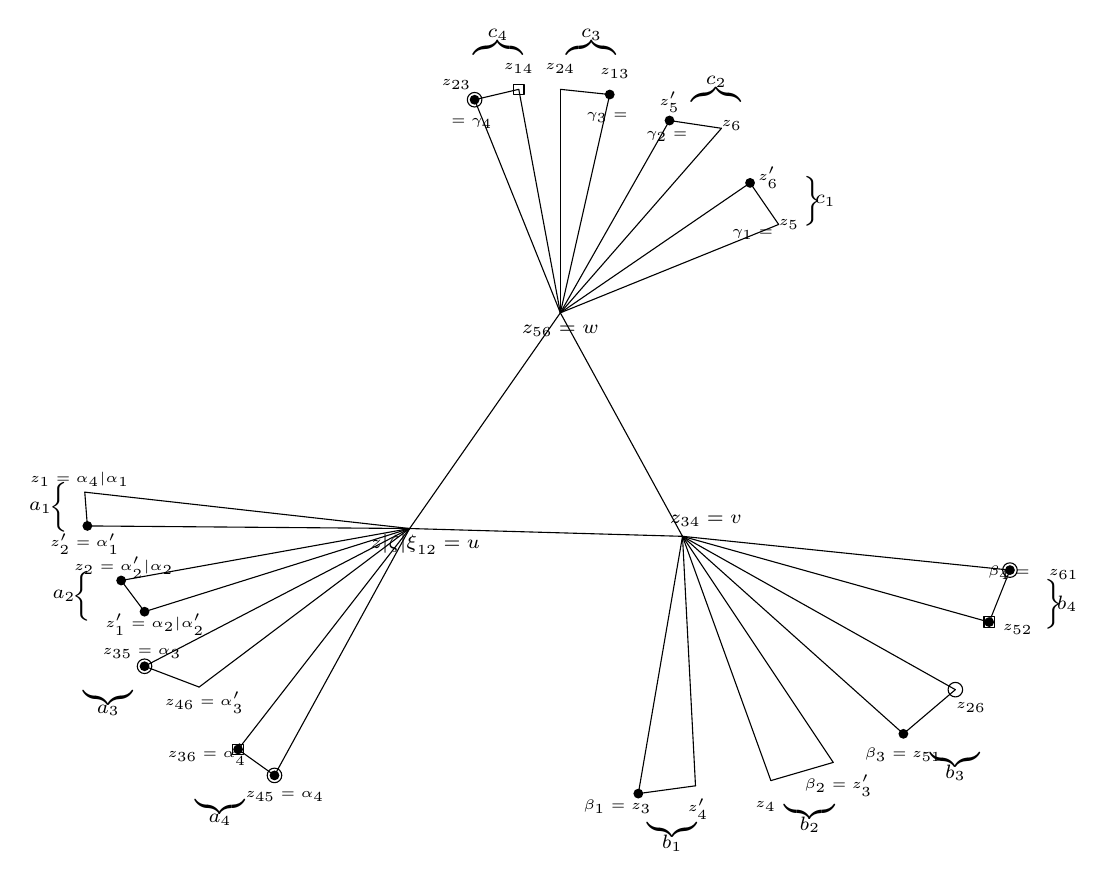
\begin{tikzpicture}[x=0.033cm,y=-0.033cm,line cap=round,line join=round,line width=.4pt]
\draw (142,165) -- (247,168) -- (200,82) -- cycle;
\node[inner sep=.55pt,anchor=center,font=\scriptsize] at (148,171) {$\unsure{z|\zeta|\xi}_{12}=u$};
\node[inner sep=.55pt,anchor=center,font=\scriptsize] at (256,162) {$z_{34}=v$};
\node[inner sep=.55pt,anchor=center,font=\scriptsize] at (200,89) {$z_{56}=w$};
\draw (142,165) -- (17,151);
\draw (142,165) -- (18,164);
\draw (17,151) -- (18,164);
\draw (142,165) -- (31,185);
\draw (142,165) -- (40,197);
\draw (31,185) -- (40,197);
\draw (142,165) -- (40,218);
\draw (142,165) -- (61,226);
\draw (40,218) -- (61,226);
\draw (142,165) -- (76,250);
\draw (142,165) -- (90,260);
\draw (76,250) -- (90,260);
\fill (18,164) circle[radius=0.0625cm];
\fill (31,185) circle[radius=0.0625cm];
\fill (40,197) circle[radius=0.0625cm];
\fill (40,218) circle[radius=0.0625cm];
\fill (76,250) circle[radius=0.0625cm];
\fill (90,260) circle[radius=0.0625cm];
\draw (74,248) -- (78,248) -- (78,252) -- (74,252) -- cycle;
\draw (40,218) circle[radius=0.0925cm];
\draw (90,260) circle[radius=0.0925cm];
\node[inner sep=.55pt,anchor=center,font=\tiny] at (15,146) {$z_1=\unsure{\alpha_4|\alpha_1}$};
\node[inner sep=.55pt,anchor=center,font=\tiny] at (17,171) {$z'_2=\alpha'_1$};
\node[inner sep=.55pt,anchor=center,font=\tiny] at (32,180) {$z_2=\unsure{\alpha'_2|\alpha_2}$};
\node[inner sep=.55pt,anchor=center,font=\tiny] at (44,202) {$z'_1=\unsure{\alpha_2|\alpha'_2}$};
\node[inner sep=.55pt,anchor=center,font=\tiny] at (39,213) {$z_{35}=\unsure{\alpha_3}$};
\node[inner sep=.55pt,anchor=center,font=\tiny] at (63,232) {$z_{46}=\unsure{\alpha'_3}$};
\node[inner sep=.55pt,anchor=center,font=\tiny] at (64,252) {$z_{36}=\alpha'_4$};
\node[inner sep=.55pt,anchor=center,font=\tiny] at (94,268) {$z_{45}=\alpha_4$};
\node[inner sep=.55pt,anchor=center,font=\scriptsize] at (0,157) {$a_1$};
\node[inner sep=.55pt,anchor=center,font=\scriptsize] at (7,157) {$\big\{$};
\node[inner sep=.55pt,anchor=center,font=\scriptsize] at (9,191) {$a_2$};
\node[inner sep=.55pt,anchor=center,font=\scriptsize] at (16,191) {$\big\{$};
\node[inner sep=.55pt,anchor=center,font=\scriptsize] at (26,235) {$a_3$};
\node[inner sep=.55pt,anchor=center,font=\tiny] at (26,230) {$\underbrace{\hphantom{abc}}$};
\node[inner sep=.55pt,anchor=center,font=\scriptsize] at (69,277) {$a_4$};
\node[inner sep=.55pt,anchor=center,font=\tiny] at (69,272) {$\underbrace{\hphantom{abc}}$};
\draw (247,168) -- (230,267);
\draw (247,168) -- (252,264);
\draw (230,267) -- (252,264);
\draw (247,168) -- (281,262);
\draw (247,168) -- (305,255);
\draw (281,262) -- (305,255);
\draw (247,168) -- (332,244);
\draw (247,168) -- (352,227);
\draw (332,244) -- (352,227);
\draw (247,168) -- (365,201);
\draw (247,168) -- (373,181);
\draw (365,201) -- (373,181);
\fill (230,267) circle[radius=0.0625cm];
\fill (332,244) circle[radius=0.0625cm];
\fill (365,201) circle[radius=0.0625cm];
\fill (373,181) circle[radius=0.0625cm];
\draw (363,199) -- (367,199) -- (367,203) -- (363,203) -- cycle;
\draw (352,227) circle[radius=0.0925cm];
\draw (373,181) circle[radius=0.0925cm];
\node[inner sep=.55pt,anchor=center,font=\tiny] at (222,272) {$\beta_1=z_3$};
\node[inner sep=.55pt,anchor=center,font=\tiny] at (253,273) {$z'_4$};
\node[inner sep=.55pt,anchor=center,font=\tiny] at (279,272) {$z_4$};
\node[inner sep=.55pt,anchor=center,font=\tiny] at (307,264) {$\beta_2=z'_3$};
\node[inner sep=.55pt,anchor=center,font=\tiny] at (332,252) {$\beta_3=z_{51}$};
\node[inner sep=.55pt,anchor=center,font=\tiny] at (358,234) {$z_{26}$};
\node[inner sep=.55pt,anchor=center,font=\tiny] at (376,204) {$z_{52}$};
\node[inner sep=.55pt,anchor=center,font=\tiny] at (382,182) {$\beta_4=\phantom{z}\,z_{61}$};
\node[inner sep=.55pt,anchor=center,font=\scriptsize] at (243,286) {$b_1$};
\node[inner sep=.55pt,anchor=center,font=\tiny] at (243,281) {$\underbrace{\hphantom{abc}}$};
\node[inner sep=.55pt,anchor=center,font=\scriptsize] at (296,279) {$b_2$};
\node[inner sep=.55pt,anchor=center,font=\tiny] at (296,274) {$\underbrace{\hphantom{abc}}$};
\node[inner sep=.55pt,anchor=center,font=\scriptsize] at (352,259) {$b_3$};
\node[inner sep=.55pt,anchor=center,font=\tiny] at (352,254) {$\underbrace{\hphantom{abc}}$};
\node[inner sep=.55pt,anchor=center,font=\scriptsize] at (395,194) {$b_4$};
\node[inner sep=.55pt,anchor=center,font=\scriptsize] at (390,194) {$\big\}$};
\draw (200,82) -- (167,0);
\draw (200,82) -- (184,-4);
\draw (167,0) -- (184,-4);
\draw (200,82) -- (200,-4);
\draw (200,82) -- (219,-2);
\draw (200,-4) -- (219,-2);
\draw (200,82) -- (242,8);
\draw (200,82) -- (262,11);
\draw (242,8) -- (262,11);
\draw (200,82) -- (273,32);
\draw (200,82) -- (284,48);
\draw (273,32) -- (284,48);
\fill (167,0) circle[radius=0.0625cm];
\fill (219,-2) circle[radius=0.0625cm];
\fill (242,8) circle[radius=0.0625cm];
\fill (273,32) circle[radius=0.0625cm];
\draw (182,-6) -- (186,-6) -- (186,-2) -- (182,-2) -- cycle;
\draw (167,0) circle[radius=0.0925cm];
\node[inner sep=.55pt,anchor=center,font=\tiny] at (160,-6) {$z_{23}$};
\node[inner sep=.55pt,anchor=center,font=\tiny] at (184,-12) {$z_{14}$};
\node[inner sep=.55pt,anchor=center,font=\tiny] at (200,-12) {$z_{24}$};
\node[inner sep=.55pt,anchor=center,font=\tiny] at (221,-10) {$z_{13}$};
\node[inner sep=.55pt,anchor=center,font=\tiny] at (242,1) {$z'_5$};
\node[inner sep=.55pt,anchor=center,font=\tiny] at (266,10) {$z_6$};
\node[inner sep=.55pt,anchor=center,font=\tiny] at (280,30) {$z'_6$};
\node[inner sep=.55pt,anchor=center,font=\tiny] at (288,48) {$z_5$};
\node[inner sep=.55pt,anchor=center,font=\scriptsize] at (176,-25) {$c_4$};
\node[inner sep=.55pt,anchor=center,font=\tiny] at (176,-20) {$\overbrace{\hphantom{abc}}$};
\node[inner sep=.55pt,anchor=center,font=\scriptsize] at (212,-25) {$c_3$};
\node[inner sep=.55pt,anchor=center,font=\tiny] at (212,-20) {$\overbrace{\hphantom{abc}}$};
\node[inner sep=.55pt,anchor=center,font=\scriptsize] at (260,-7) {$c_2$};
\node[inner sep=.55pt,anchor=center,font=\tiny] at (260,-2) {$\overbrace{\hphantom{abc}}$};
\node[inner sep=.55pt,anchor=center,font=\scriptsize] at (302,39) {$c_1$};
\node[inner sep=.55pt,anchor=center,font=\scriptsize] at (297,39) {$\big\}$};
\node[inner sep=.55pt,anchor=center,font=\tiny] at (166,9) {$=\gamma_4$};
\node[inner sep=.55pt,anchor=center,font=\tiny] at (218,7) {$\gamma_3=$};
\node[inner sep=.55pt,anchor=center,font=\tiny] at (241,14) {$\gamma_2=$};
\node[inner sep=.55pt,anchor=center,font=\tiny] at (274,52) {$\gamma_1=$};
\end{tikzpicture}%
}}
\end{tikzcd}%
}

\[
\begin{aligned}
a_1+a_4&=\alpha_1\\
a_2+a_4&=\alpha_2\\
a_3+a_4&=\alpha_3
\end{aligned}
\]

\diagram{%
\begin{tikzcd}[ampersand replacement=\&,column sep=0pt,row sep=0pt]
|[inner sep=0pt]| \vcenter{\hbox{%
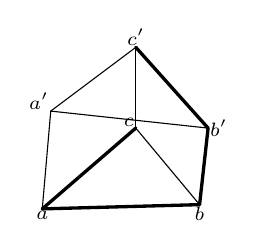
\begin{tikzpicture}[x=0.054cm,y=-0.054cm,line cap=round,line join=round,line width=.4pt]
\draw[very thick] (1,39) -- (38,38);
\draw (38,38) -- (23,20);
\draw[very thick] (23,20) -- (1,39);
\draw (3,16) -- (40,20);
\draw[very thick] (40,20) -- (23,1);
\draw (23,1) -- (3,16);
\draw (1,39) -- (3,16);
\draw[very thick] (38,38) -- (40,20);
\draw (23,20) -- (23,1);
\node[inner sep=.55pt,anchor=north,font=\scriptsize] at (1,39) {$a$};
\node[inner sep=.55pt,anchor=north,font=\scriptsize] at (38,38) {$b$};
\node[inner sep=.55pt,anchor=south east,font=\scriptsize] at (23,20) {$c$};
\node[inner sep=.55pt,anchor=south east,font=\scriptsize] at (3,16) {$a'$};
\node[inner sep=.55pt,anchor=west,font=\scriptsize] at (40,20) {$b'$};
\node[inner sep=.55pt,anchor=south,font=\scriptsize] at (23,1) {$c'$};
\end{tikzpicture}%
}}
\end{tikzcd}%
}

\unsure{prismes épinglés)|prismes épinglés}

\[
\begin{aligned}
27\cdot10\cdot8\cdot4\cdot\underline{1}&=[W]:6\\
\text{prismes}:&\quad[W]:72
\end{aligned}
\]

\diagram{%
\begin{tikzcd}[ampersand replacement=\&,column sep=0pt,row sep=0pt]
|[inner sep=0pt]| \vcenter{\hbox{%
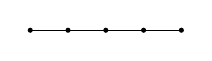
\begin{tikzpicture}[x=0.04cm,y=-0.04cm,line cap=round,line join=round,line width=.4pt]
\draw (0,0) -- (12,0) -- (24,0) -- (36,0) -- (48,0);
\fill (0,0) circle[radius=0.0325cm];
\fill (12,0) circle[radius=0.0325cm];
\fill (24,0) circle[radius=0.0325cm];
\fill (36,0) circle[radius=0.0325cm];
\fill (48,0) circle[radius=0.0325cm];
\end{tikzpicture}%
}}
\end{tikzcd}%
}

\[
\begin{aligned}
&27\cdot10\cdot8\cdot4\cdot1\\
A_5\ \text{épinglés}:&\quad[W]:6\\
A_5:&\quad[W]:12
\end{aligned}
\]

\diagram{%
\begin{tikzcd}[ampersand replacement=\&,column sep=0pt,row sep=0pt]
|[inner sep=0pt]| \vcenter{\hbox{%
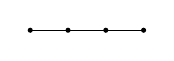
\begin{tikzpicture}[x=0.04cm,y=-0.04cm,line cap=round,line join=round,line width=.4pt]
\draw (0,0) -- (12,0) -- (24,0) -- (36,0);
\fill (0,0) circle[radius=0.0325cm];
\fill (12,0) circle[radius=0.0325cm];
\fill (24,0) circle[radius=0.0325cm];
\fill (36,0) circle[radius=0.0325cm];
\end{tikzpicture}%
}}
\end{tikzcd}%
}

\[
\begin{aligned}
A_4\ \text{épinglés}:&\quad27\cdot10\cdot8^{\inserted{4}}=[W]:\unsure{6}\\
A_4&\quad[W]:12
\end{aligned}
\]

\diagram{%
\begin{tikzcd}[ampersand replacement=\&,column sep=0pt,row sep=0pt]
|[inner sep=0pt]| \vcenter{\hbox{%
\begin{tikzpicture}[x=0.04cm,y=-0.04cm,line cap=round,line join=round,line width=.4pt]
\draw (0,0) -- (12,0) -- (24,0);
\fill (0,0) circle[radius=0.0325cm];
\fill (12,0) circle[radius=0.0325cm];
\fill (24,0) circle[radius=0.0325cm];
\end{tikzpicture}%
}}
\end{tikzcd}%
}

\[
\begin{aligned}
A_3\ \text{épinglés}:&\quad27\cdot10\cdot8=\unsure{[W]|[\mathrm{W}]}:24\\
&\text{(autres que des triangles épinglés)}\\
A_3\ \deleted{\unsure{\text{ép.}}}:&\quad[W]/48
\end{aligned}
\]

\diagram{%
\begin{tikzcd}[ampersand replacement=\&,column sep=0pt,row sep=0pt]
|[inner sep=0pt]| \vcenter{\hbox{%
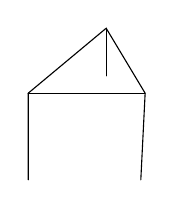
\begin{tikzpicture}[x=0.055cm,y=-0.055cm,line cap=round,line join=round,line width=.4pt]
\draw (0,35) -- (0,15) -- (18,0) -- (27,15) -- (26,35);
\draw (0,15) -- (27,15);
\draw (18,0) -- (18,11);
\end{tikzpicture}%
}}
\end{tikzcd}%
}

carroussels \inserted{simples} épinglés

\[27\cdot10\cdot8\cdot4\cdot3=[W]:2\]

carroussels \inserted{simples}\quad $[W]:12$

\diagram{%
\begin{tikzcd}[ampersand replacement=\&,column sep=0pt,row sep=0pt]
|[inner sep=0pt]| \vcenter{\hbox{%
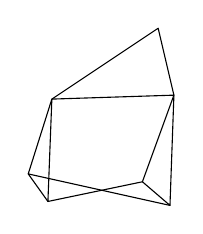
\begin{tikzpicture}[x=0.05cm,y=-0.05cm,line cap=round,line join=round,line width=.4pt]
\draw (5,37) -- (11,18) -- (38,0) -- (42,17) -- (41,45) -- (5,37);
\draw (11,18) -- (42,17) -- (34,39) -- (10,44) -- (11,18);
\draw (34,39) -- (41,45);
\draw (5,37) -- (10,44);
\end{tikzpicture}%
}}
\end{tikzcd}%
}

\unsure{$1$}

% archive sheet number: 84
\scanpage{86}

% Handwritten graphs read with binding at the top; preprinted staff ruling.

\diagram{%
\begin{tikzcd}[ampersand replacement=\&,column sep=0pt,row sep=0pt]
|[inner sep=0pt]| \vcenter{\hbox{%
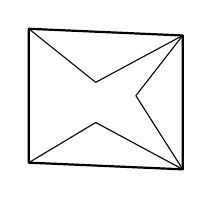
\begin{tikzpicture}[x=0.085cm,y=-0.085cm,line cap=round,line join=round,line width=.4pt]
\draw[thick] (0,0) -- (23,1) -- (23,21) -- (0,20) -- cycle;
\draw (0,0) -- (10,8) -- (23,1);
\draw (23,1) -- (16,10) -- (23,21);
\draw (23,21) -- (10,14) -- (0,20);
\end{tikzpicture}%
}}
\end{tikzcd}%
}

\diagram{%
\begin{tikzcd}[ampersand replacement=\&,column sep=0pt,row sep=0pt]
|[inner sep=0pt]| \vcenter{\hbox{%
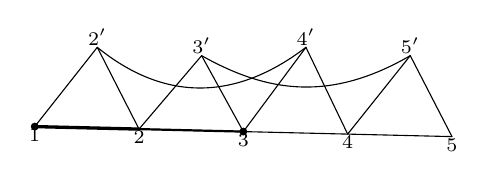
\begin{tikzpicture}[x=0.053cm,y=-0.053cm,line cap=round,line join=round,line width=.4pt]
\draw (0,20.0) -- (25,20.6) -- (50,21.2) -- (75,21.8) -- (100,22.4);
\draw (0,20.0) -- (15,1) -- (25,20.6);
\node[inner sep=.55pt,anchor=south,font=\scriptsize] at (15,1) {$2'$};
\draw (25,20.6) -- (40,3) -- (50,21.2);
\node[inner sep=.55pt,anchor=south,font=\scriptsize] at (40,3) {$3'$};
\draw (50,21.2) -- (65,1) -- (75,21.8);
\node[inner sep=.55pt,anchor=south,font=\scriptsize] at (65,1) {$4'$};
\draw (75,21.8) -- (90,3) -- (100,22.4);
\node[inner sep=.55pt,anchor=south,font=\scriptsize] at (90,3) {$5'$};
\node[inner sep=.55pt,anchor=north,font=\scriptsize] at (0,20.0) {$1$};
\node[inner sep=.55pt,anchor=north,font=\scriptsize] at (25,20.6) {$2$};
\node[inner sep=.55pt,anchor=north,font=\scriptsize] at (50,21.2) {$3$};
\node[inner sep=.55pt,anchor=north,font=\scriptsize] at (75,21.8) {$4$};
\node[inner sep=.55pt,anchor=north,font=\scriptsize] at (100,22.4) {$5$};
\draw (15,1) .. controls (31,14) and (48,14) .. (65,1);
\draw (40,3) .. controls (56,12) and (71,14) .. (90,3);
\draw[very thick] (0,20.0) -- (25,20.6);
\draw[thick] (25,20.6) -- (50,21.2);
\fill (0,20.0) circle[radius=0.05cm];
\fill (50,21.2) circle[radius=0.05cm];
\end{tikzpicture}%
}}
\end{tikzcd}%
}

\diagram{%
\begin{tikzcd}[ampersand replacement=\&,column sep=0pt,row sep=0pt]
|[inner sep=0pt]| \vcenter{\hbox{%
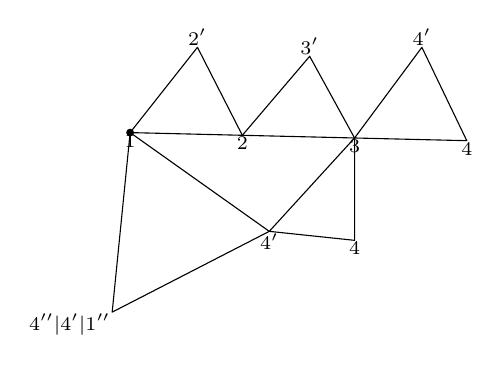
\begin{tikzpicture}[x=0.057cm,y=-0.057cm,line cap=round,line join=round,line width=.4pt]
\draw (0,20.0) -- (25,20.6) -- (50,21.2) -- (75,21.8);
\draw (0,20.0) -- (15,1) -- (25,20.6);
\node[inner sep=.55pt,anchor=south,font=\scriptsize] at (15,1) {$2'$};
\draw (25,20.6) -- (40,3) -- (50,21.2);
\node[inner sep=.55pt,anchor=south,font=\scriptsize] at (40,3) {$3'$};
\draw (50,21.2) -- (65,1) -- (75,21.8);
\node[inner sep=.55pt,anchor=south,font=\scriptsize] at (65,1) {$4'$};
\node[inner sep=.55pt,anchor=north,font=\scriptsize] at (0,20.0) {$1$};
\node[inner sep=.55pt,anchor=north,font=\scriptsize] at (25,20.6) {$2$};
\node[inner sep=.55pt,anchor=north,font=\scriptsize] at (50,21.2) {$3$};
\node[inner sep=.55pt,anchor=north,font=\scriptsize] at (75,21.8) {$4$};
\node[inner sep=.55pt,anchor=south,font=\scriptsize] at (65,1) {$\phantom{4'}$};
\draw (0,20.0) -- (-4,60) -- (31,42) -- (0,20.0);
\draw (31,42) -- (50,21.2) -- (50,44) -- cycle;
\node[inner sep=.55pt,anchor=north east,font=\scriptsize] at (-4,60) {$\unsure{4''|4'|1''}$};
\node[inner sep=.55pt,anchor=north,font=\scriptsize] at (31,42) {$4'$};
\node[inner sep=.55pt,anchor=north,font=\scriptsize] at (50,44) {$4$};
\fill (0,20.0) circle[radius=0.05cm];
\end{tikzpicture}%
}}
\end{tikzcd}%
}

\diagram{%
\begin{tikzcd}[ampersand replacement=\&,column sep=0pt,row sep=0pt]
|[inner sep=0pt]| \vcenter{\hbox{%
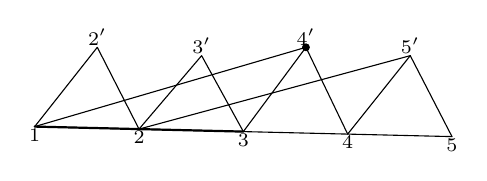
\begin{tikzpicture}[x=0.053cm,y=-0.053cm,line cap=round,line join=round,line width=.4pt]
\draw (0,20.0) -- (25,20.6) -- (50,21.2) -- (75,21.8) -- (100,22.4);
\draw (0,20.0) -- (15,1) -- (25,20.6);
\node[inner sep=.55pt,anchor=south,font=\scriptsize] at (15,1) {$2'$};
\draw (25,20.6) -- (40,3) -- (50,21.2);
\node[inner sep=.55pt,anchor=south,font=\scriptsize] at (40,3) {$3'$};
\draw (50,21.2) -- (65,1) -- (75,21.8);
\node[inner sep=.55pt,anchor=south,font=\scriptsize] at (65,1) {$4'$};
\draw (75,21.8) -- (90,3) -- (100,22.4);
\node[inner sep=.55pt,anchor=south,font=\scriptsize] at (90,3) {$5'$};
\node[inner sep=.55pt,anchor=north,font=\scriptsize] at (0,20.0) {$1$};
\node[inner sep=.55pt,anchor=north,font=\scriptsize] at (25,20.6) {$2$};
\node[inner sep=.55pt,anchor=north,font=\scriptsize] at (50,21.2) {$3$};
\node[inner sep=.55pt,anchor=north,font=\scriptsize] at (75,21.8) {$4$};
\node[inner sep=.55pt,anchor=north,font=\scriptsize] at (100,22.4) {$5$};
\draw (0,20.0) -- (65,1);
\draw (25,20.6) -- (90,3);
\draw[thick] (0,20.0) -- (50,21.2);
\fill (65,1) circle[radius=0.05cm];
\end{tikzpicture}%
}}
\end{tikzcd}%
}

\diagram{%
\begin{tikzcd}[ampersand replacement=\&,column sep=0pt,row sep=0pt]
|[inner sep=0pt]| \vcenter{\hbox{%
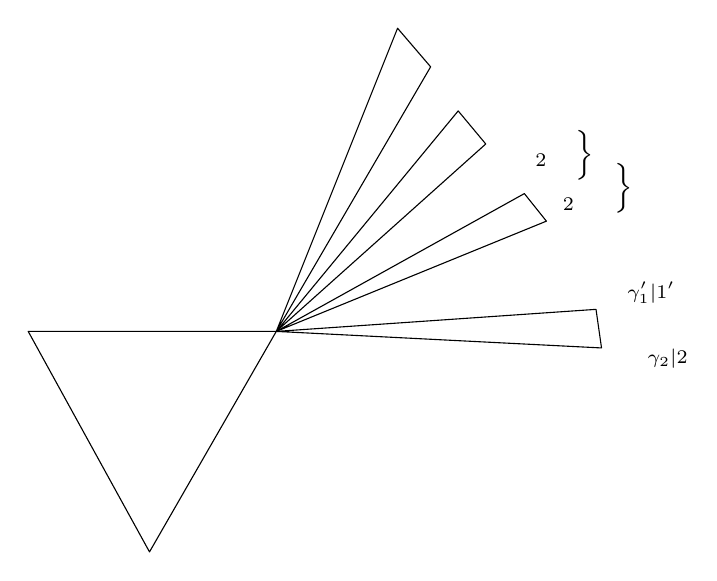
\begin{tikzpicture}[x=0.07cm,y=-0.07cm,line cap=round,line join=round,line width=.4pt]
\draw (-45,0) -- (-23,40) -- (0,0) -- cycle;
\draw (0,0) -- (22,-55) -- (28,-48) -- cycle;
\draw (0,0) -- (33,-40) -- (38,-34) -- cycle;
\draw (0,0) -- (45,-25) -- (49,-20) -- cycle;
\draw (0,0) -- (58,-4) -- (59,3) -- cycle;
\node[inner sep=.55pt,anchor=center,font=\scriptsize] at (48,-31) {$\unsure{2}$};
\node[inner sep=.55pt,anchor=center,font=\scriptsize] at (53,-23) {$\unsure{2}$};
\node[inner sep=.55pt,anchor=center,font=\scriptsize] at (56,-32) {$\big\}$};
\node[inner sep=.55pt,anchor=center,font=\scriptsize] at (63,-26) {$\big\}$};
\node[inner sep=.55pt,anchor=center,font=\scriptsize] at (68,-7) {$\unsure{\gamma'_1|1'}$};
\node[inner sep=.55pt,anchor=center,font=\scriptsize] at (71,5) {$\unsure{\gamma_2|2}$};
\end{tikzpicture}%
}}
\end{tikzcd}%
}

% archive sheet number: 85
\scanpage{87}

\[
\begin{aligned}
&\unsure{z|\zeta|\xi}_1\quad z_{14}\quad z_4\quad z'_2\\
&z_1\,\big|\,z'_2\ z'_3\ z_{31}\ z_{12}
\end{aligned}
\]

\diagram{%
\begin{tikzcd}[ampersand replacement=\&,column sep=0pt,row sep=0pt]
|[inner sep=0pt]| \vcenter{\hbox{%
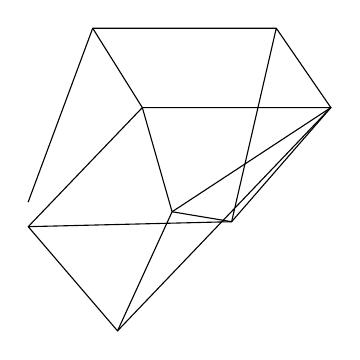
\begin{tikzpicture}[x=0.063cm,y=-0.063cm,line cap=round,line join=round,line width=.4pt]
\draw (0,36) -- (13,1) -- (50,1) -- (61,17) -- (18,62) -- (0,41) -- (41,40) -- (50,1);
\draw (13,1) -- (23,17) -- (61,17);
\draw (0,41) -- (23,17) -- (29,38) -- (61,17);
\draw (18,62) -- (29,38) -- (41,40) -- (61,17);
\end{tikzpicture}%
}}
\end{tikzcd}%
}

\diagram{%
\begin{tikzcd}[ampersand replacement=\&,column sep=0pt,row sep=0pt]
|[inner sep=0pt]| \vcenter{\hbox{%
\begin{tikzpicture}[x=0.066cm,y=-0.066cm,line cap=round,line join=round,line width=.4pt]
\draw[thick] (0,0) -- (0,18);
\draw (0,0) -- (26,18) -- (26,0);
\draw (1,22) -- (3,39);
\draw (26,21) -- (29,39);
\node[inner sep=.55pt,anchor=center,font=\scriptsize] at (-4,9) {$\delta$};
\node[inner sep=.55pt,anchor=center,font=\scriptsize] at (16,3) {$\delta'$};
\node[inner sep=.55pt,anchor=center,font=\scriptsize] at (34,8) {$\delta''$};
\node[inner sep=.55pt,anchor=center,font=\scriptsize] at (-6,30) {$\delta'''$};
\node[inner sep=.55pt,anchor=center,font=\scriptsize] at (35,27) {$\delta^{\mathrm{IV}}$};
\fill (48,2) circle[radius=0.0225cm];
\fill (52,18) circle[radius=0.0225cm];
\fill (52,39) circle[radius=0.0225cm];
\fill (65,8) circle[radius=0.0225cm];
\fill (65,18) circle[radius=0.0225cm];
\fill (65,39) circle[radius=0.0225cm];
\end{tikzpicture}%
}}
\end{tikzcd}%
}

\[
\begin{aligned}
\delta&=z_1,\quad\delta'=z_2,\quad\delta''=\unsure{z'_2|J'_2|\xi'_2}\\
\delta'''&=z_{14}\quad\delta^{\mathrm{IV}}=z_{25}
\end{aligned}\qquad
\begin{aligned}
\delta\delta'&=0&\delta\delta''&=1\\
\delta\delta'''&=1&\delta\delta^{\mathrm{IV}}&=0
\end{aligned}
\]

\diagram{%
\begin{tikzcd}[ampersand replacement=\&,column sep=0pt,row sep=0pt]
|[inner sep=0pt]| \vcenter{\hbox{%
\begin{tikzpicture}[x=0.06cm,y=-0.06cm,line cap=round,line join=round,line width=.4pt]
\draw (0,0) -- (0,24);
\fill (0,12) circle[radius=0.05cm];
\end{tikzpicture}%
}}
\end{tikzcd}%
}

\[
\delta\delta'\ \deleted{\bmod 2}\equiv\operatorname{card}(\delta\cap\delta')+\operatorname{card}(\varepsilon(\delta)\cap\varepsilon(\delta'))
\]

\diagram{%
\begin{tikzcd}[ampersand replacement=\&,column sep=0pt,row sep=0pt]
|[inner sep=0pt]| \vcenter{\hbox{%
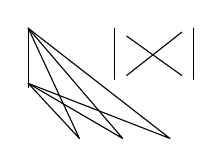
\begin{tikzpicture}[x=0.05cm,y=-0.05cm,line cap=round,line join=round,line width=.4pt]
\draw (0,0) -- (0,15);
\draw (0,0) -- (13,28) -- (0,14);
\draw (0,0) -- (24,28) -- (0,14);
\draw (0,0) -- (36,28) -- (0,14);
\draw (22,0) -- (22,13);
\draw (42,0) -- (42,13);
\draw (25,2) -- (39,12);
\draw (25,12) -- (39,1);
\end{tikzpicture}%
}}
\end{tikzcd}%
}

\diagram{%
\begin{tikzcd}[ampersand replacement=\&,column sep=0pt,row sep=0pt]
|[inner sep=0pt]| \vcenter{\hbox{%
\begin{tikzpicture}[x=0.05cm,y=-0.05cm,line cap=round,line join=round,line width=.4pt]
\draw (0,0) -- (1,14);
\draw (11,0) -- (12,14);
\draw (23,0) -- (23,29);
\draw (1,16) -- (-1,29) -- (2,27);
\draw (1,37) -- (1,46);
\end{tikzpicture}%
}}
\end{tikzcd}%
}

\diagram{%
\begin{tikzcd}[ampersand replacement=\&,column sep=0pt,row sep=0pt]
|[inner sep=0pt]| \vcenter{\hbox{%
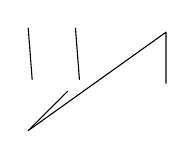
\begin{tikzpicture}[x=0.05cm,y=-0.05cm,line cap=round,line join=round,line width=.4pt]
\draw (0,0) -- (1,13);
\draw (12,0) -- (13,13);
\draw (0,26) -- (35,1) -- (35,14);
\draw (0,26) -- (10,16);
\end{tikzpicture}%
}}
\end{tikzcd}%
}

\diagram{%
\begin{tikzcd}[ampersand replacement=\&,column sep=0pt,row sep=0pt]
|[inner sep=0pt]| \vcenter{\hbox{%
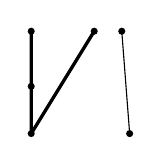
\begin{tikzpicture}[x=0.05cm,y=-0.05cm,line cap=round,line join=round,line width=.4pt]
\draw[very thick] (0,0) -- (0,26) -- (16,0);
\draw (23,0) -- (25,26);
\fill (0,0) circle[radius=0.045cm];
\fill (0,14) circle[radius=0.045cm];
\fill (0,26) circle[radius=0.045cm];
\fill (16,0) circle[radius=0.045cm];
\fill (23,0) circle[radius=0.045cm];
\fill (25,26) circle[radius=0.045cm];
\end{tikzpicture}%
}}
\end{tikzcd}%
}

\diagram{%
\begin{tikzcd}[ampersand replacement=\&,column sep=0pt,row sep=0pt]
|[inner sep=0pt]| \vcenter{\hbox{%
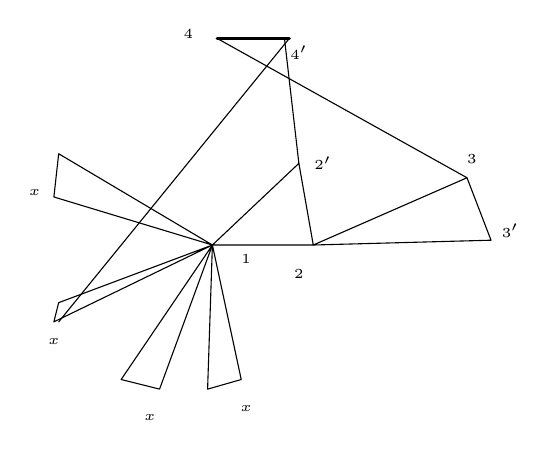
\begin{tikzpicture}[x=0.061cm,y=-0.061cm,line cap=round,line join=round,line width=.4pt]
\draw (33,44) -- (0,34) -- (1,25) -- cycle;
\draw (33,44) -- (0,60) -- (1,56) -- cycle;
\draw (33,44) -- (14,72) -- (22,74) -- cycle;
\draw (33,44) -- (32,74) -- (39,72) -- cycle;
\draw (33,44) -- (54,44) -- (51,27) -- cycle;
\draw (54,44) -- (86,30) -- (91,43) -- cycle;
\draw (1,60) -- (49,1) -- (34,1) -- (86,30);
\draw[very thick] (34,1) -- (49,1);
\draw (48,1) -- (51,27);
\node[inner sep=.55pt,anchor=center,font=\tiny] at (-4,33) {$x$};
\node[inner sep=.55pt,anchor=center,font=\tiny] at (0,64) {$x$};
\node[inner sep=.55pt,anchor=center,font=\tiny] at (20,80) {$x$};
\node[inner sep=.55pt,anchor=center,font=\tiny] at (40,78) {$x$};
\node[inner sep=.55pt,anchor=center,font=\tiny] at (40,47) {$1$};
\node[inner sep=.55pt,anchor=center,font=\tiny] at (51,50) {$2$};
\node[inner sep=.55pt,anchor=center,font=\tiny] at (56,27) {$2'$};
\node[inner sep=.55pt,anchor=center,font=\tiny] at (87,26) {$3$};
\node[inner sep=.55pt,anchor=center,font=\tiny] at (95,41) {$3'$};
\node[inner sep=.55pt,anchor=center,font=\tiny] at (28,0) {$4$};
\node[inner sep=.55pt,anchor=center,font=\tiny] at (51,4) {$\unsure{4'}$};
\end{tikzpicture}%
}}
\end{tikzcd}%
}

\unsure{hexagone|hexagones} pointés orientés

\[
\underbrace{27}\cdot10\cdot\underbrace{8\cdot4}\cdot1\cdot\underbrace{1}
=2^6\cdot3^{\unsure{3|2}}\cdot5=[W]:6
\]

hexagones : $[W]:72$

\diagram{%
\begin{tikzcd}[ampersand replacement=\&,column sep=0pt,row sep=0pt]
|[inner sep=0pt]| \vcenter{\hbox{%
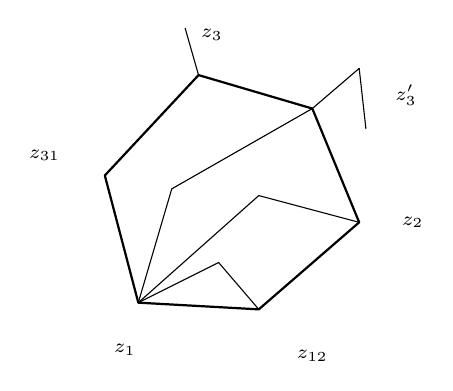
\begin{tikzpicture}[x=0.085cm,y=-0.085cm,line cap=round,line join=round,line width=.4pt]
\draw[thick] (0,22) -- (14,7) -- (31,12) -- (38,29) -- (23,42) -- (5,41) -- cycle;
\draw (14,7) -- (12,0);
\draw (31,12) -- (38,6) -- (39,15);
\draw (5,41) -- (10,24) -- (31,12);
\draw (5,41) -- (23,25) -- (38,29);
\draw (5,41) -- (17,35) -- (23,42);
\node[inner sep=.55pt,anchor=center,font=\scriptsize] at (-9,19) {$z_{31}$};
\node[inner sep=.55pt,anchor=center,font=\scriptsize] at (16,1) {$z_3$};
\node[inner sep=.55pt,anchor=center,font=\scriptsize] at (45,10) {$z'_3$};
\node[inner sep=.55pt,anchor=center,font=\scriptsize] at (46,29) {$z_2$};
\node[inner sep=.55pt,anchor=center,font=\scriptsize] at (31,49) {$z_{12}$};
\node[inner sep=.55pt,anchor=center,font=\scriptsize] at (3,48) {$z_1$};
\end{tikzpicture}%
}}
\end{tikzcd}%
}

\diagram{%
\begin{tikzcd}[ampersand replacement=\&,column sep=0pt,row sep=0pt]
|[inner sep=0pt]| \vcenter{\hbox{%
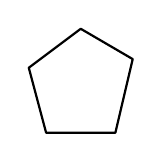
\begin{tikzpicture}[x=0.055cm,y=-0.055cm,line cap=round,line join=round,line width=.4pt]
\draw[thick] (0,9) -- (12,0) -- (24,7) -- (20,24) -- (4,24) -- cycle;
\end{tikzpicture}%
}}
\end{tikzcd}%
}

pentagones pointés orientés

\[27\cdot10\cdot8\cdot4\cdot3\overset{\displaystyle=2^6 3^4 5}{=}[W]:2\]

pentagones \quad $[W]:20$

\[
\begin{aligned}
\text{\unsure{carré|carrés} pointés}\quad&27\cdot10\cdot8\cdot4=[W]:6\\
\text{carrés}:&\ [W]:48
\end{aligned}
\]

\[\mathbb F_2^{\unsure{4|i}}\quad\vert\]

\diagram{%
\begin{tikzcd}[ampersand replacement=\&,column sep=0pt,row sep=0pt]
|[inner sep=0pt]| \vcenter{\hbox{%
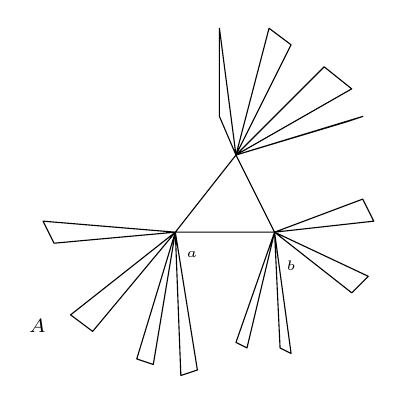
\begin{tikzpicture}[x=0.07cm,y=-0.07cm,line cap=round,line join=round,line width=.4pt]
\draw (15,28) -- (33,28) -- (26,14) -- cycle;
\draw (26,14) -- (23,-9) -- (23,7) -- cycle;
\draw (26,14) -- (32,-9) -- (36,-6) -- cycle;
\draw (26,14) -- (42,-2) -- (47,2) -- cycle;
\draw (26,14) -- (46,8) -- (49,7) -- cycle;
\draw (15,28) -- (-9,26) -- (-7,30) -- cycle;
\draw (15,28) -- (-4,43) -- (0,46) -- cycle;
\draw (15,28) -- (8,51) -- (11,52) -- cycle;
\draw (15,28) -- (16,54) -- (19,53) -- cycle;
\draw (33,28) -- (51,26) -- (49,22) -- cycle;
\draw (33,28) -- (47,39) -- (50,36) -- cycle;
\draw (33,28) -- (34,49) -- (36,50) -- cycle;
\draw (33,28) -- (26,48) -- (28,49) -- cycle;
\node[inner sep=.55pt,anchor=center,font=\scriptsize] at (-10,45) {$A$};
\node[inner sep=.55pt,anchor=center,font=\tiny] at (18,32) {$a$};
\node[inner sep=.55pt,anchor=center,font=\tiny] at (36,34) {$b$};
\end{tikzpicture}%
}}
\end{tikzcd}%
}

\[
\text{\unsure{Calculons|Combien|Conditions}\ \operatorname{card}}\quad |\{z\in\widetilde A\quad\text{\unsure{z lié à x.|$\xi$ liés à $x$}}\]
\[\lambda_{12}\quad\lambda_{23}\quad\lambda_{4\unsure{\cdot}}\]

\[
\begin{aligned}
\mathbb F_2^A&\ \mathrm P\\[-2pt]
&x,y\qquad x-y=u\in\mathbb F_2^A\simeq\mathscr P(A)
\end{aligned}
\]

former les $\alpha\in A$ sur lesquels $\operatorname{Et}(x)\cap\widetilde A$ \inserted{et $\operatorname{Et}(y)\cap\widetilde A$} \deleted{\unsure{coïncident}} sont distincts

\[
x,y\ \text{liés}\Longleftrightarrow
\left\{\begin{aligned}
&x\text{ et }y\text{ de même parité},\quad \text{i.e. card }u\text{ paire}:\\
&\quad x-y=\mathbf1\ \unsure{=A|{}^{A}}\quad
 (\operatorname{Et}(x)\cap\widetilde A\text{ et }\operatorname{Et}(y)\cap\widetilde A\text{ sont complémentaires})\\
&\text{\unsure{pour}}\quad x\text{ et }y\text{ de parité }\unsure{\ne|\text{contr.}},\quad\text{i.e. card }u\text{ impaire}:\\
&\quad\deleted{\unsure{x-y}}\quad \underline{\operatorname{card}u=3}
\end{aligned}\right.
\]

\[
\underline{x,y\ \text{non liés}}\Longleftrightarrow
\left\{\begin{aligned}
&x\text{ et }y\text{ de même parité i.e. card }u\text{ paire}:\quad x-y\ne\mathbf 1\\
&\quad\text{i.e. }(\operatorname{Et}(x)\cap\widetilde A)\cap\operatorname{Et}(y)\cap\widetilde A\ne\varnothing\\
&x\text{ et }y\text{ de parité contr.}:\quad\operatorname{card}u=1\\
&\quad\text{i.e. card }u\text{ impaire}
\end{aligned}\right.
\]

\diagram{%
\begin{tikzcd}[ampersand replacement=\&,column sep=0pt,row sep=0pt]
|[inner sep=0pt]| \vcenter{\hbox{%
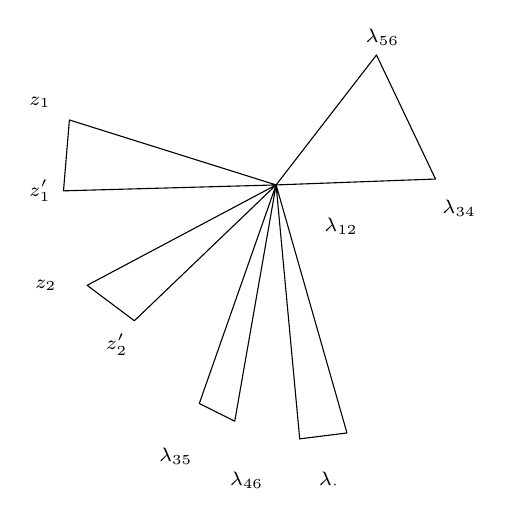
\begin{tikzpicture}[x=0.075cm,y=-0.075cm,line cap=round,line join=round,line width=.4pt]
\draw (35,22) -- (52,0) -- (62,21) -- cycle;
\draw (35,22) -- (0,11) -- (-1,23) -- cycle;
\draw (35,22) -- (3,39) -- (11,45) -- cycle;
\draw (35,22) -- (22,59) -- (28,62) -- cycle;
\draw (35,22) -- (39,65) -- (47,64) -- cycle;
\node[inner sep=.55pt,anchor=center,font=\scriptsize] at (53,-3) {$\lambda_{56}$};
\node[inner sep=.55pt,anchor=center,font=\scriptsize] at (66,26) {$\lambda_{34}$};
\node[inner sep=.55pt,anchor=center,font=\scriptsize] at (46,29) {$\lambda_{12}$};
\node[inner sep=.55pt,anchor=center,font=\scriptsize] at (-5,8) {$z_1$};
\node[inner sep=.55pt,anchor=center,font=\scriptsize] at (-5,23) {$z'_1$};
\node[inner sep=.55pt,anchor=center,font=\scriptsize] at (-4,39) {$z_2$};
\node[inner sep=.55pt,anchor=center,font=\scriptsize] at (8,49) {$z'_2$};
\node[inner sep=.55pt,anchor=center,font=\scriptsize] at (18,68) {$\lambda_{35}$};
\node[inner sep=.55pt,anchor=center,font=\scriptsize] at (30,72) {$\lambda_{46}$};
\node[inner sep=.55pt,anchor=center,font=\scriptsize] at (44,72) {$\lambda_{\unsure{\cdot}}$};
\end{tikzpicture}%
}}
\end{tikzcd}%
}

\[
\begin{aligned}
x,y\ \text{liés}&\Longleftrightarrow\operatorname{card}u=3\text{ ou }4\\
x,y\ \text{non liés}&\Longleftrightarrow\operatorname{card}u=\underset{(x=y)}{0},1\text{ ou }2
\end{aligned}
\]

\diagram{%
\begin{tikzcd}[ampersand replacement=\&,column sep=0pt,row sep=0pt]
|[inner sep=0pt]| \vcenter{\hbox{%
\begin{tikzpicture}[x=0.065cm,y=-0.065cm,line cap=round,line join=round,line width=.4pt]
\draw (9,0) -- (51,49);
\draw (0,8) -- (5,18);
\fill (5,18) circle[radius=0.0325cm];
\draw (10,23) -- (18,33);
\fill (18,33) circle[radius=0.0325cm];
\draw (22,36) -- (31,46);
\fill (31,46) circle[radius=0.0325cm];
\draw (35,50) -- (42,57);
\fill (42,57) circle[radius=0.0325cm];
\draw (18,0) -- (23,9);
\fill (23,9) circle[radius=0.0325cm];
\draw (27,15) -- (34,24);
\fill (34,24) circle[radius=0.0325cm];
\draw (39,29) -- (45,38);
\fill (45,38) circle[radius=0.0325cm];
\draw (50,43) -- (57,51);
\fill (57,51) circle[radius=0.0325cm];
\node[inner sep=.55pt,anchor=center,font=\tiny] at (0,8) {$+$};
\node[inner sep=.55pt,anchor=center,font=\tiny] at (18,33) {$+$};
\node[inner sep=.55pt,anchor=center,font=\tiny] at (31,46) {$+$};
\node[inner sep=.55pt,anchor=center,font=\tiny] at (42,57) {$+$};
\node[inner sep=.55pt,anchor=center,font=\tiny] at (18,0) {$+$};
\node[inner sep=.55pt,anchor=center,font=\tiny] at (34,24) {$+$};
\node[inner sep=.55pt,anchor=center,font=\tiny] at (45,38) {$+$};
\node[inner sep=.55pt,anchor=center,font=\tiny] at (57,51) {$+$};
\end{tikzpicture}%
}}
\end{tikzcd}%
}

\[
\begin{aligned}
\text{triangles pointés orientés}\quad&27\cdot10=270=[W]:\unsure{2^6\cdot3^1|2^3\cdot3^4}\\
\text{triangles}:\quad&\frac{27\cdot10}{6}=45=[W]:2^7\cdot3^2
\end{aligned}
\]

% archive sheet number: 86
\scanpage{88}

\diagram{%
\begin{tikzcd}[ampersand replacement=\&,column sep=0pt,row sep=0pt]
|[inner sep=0pt]| \vcenter{\hbox{%
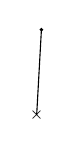
\begin{tikzpicture}[x=0.06cm,y=-0.06cm,line cap=round,line join=round,line width=.4pt]
\draw (1,0) -- (0,18);
\fill (1,0) circle[radius=0.025cm];
\node[inner sep=.55pt,anchor=center,font=\tiny] at (0,18) {$\times$};
\end{tikzpicture}%
}}
\end{tikzcd}%
}

\diagram{%
\begin{tikzcd}[ampersand replacement=\&,column sep=0pt,row sep=0pt]
|[inner sep=0pt]| \vcenter{\hbox{%
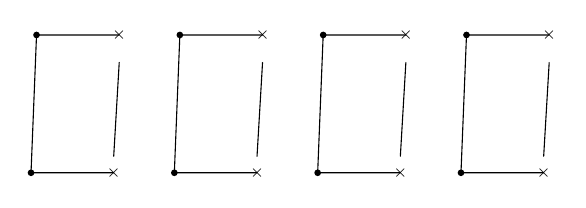
\begin{tikzpicture}[x=0.07cm,y=-0.07cm,line cap=round,line join=round,line width=.4pt]
\draw (15,0) -- (0,0) -- (-1,25) -- (14,25);
\draw (15,5) -- (14,22);
\fill (0,0) circle[radius=0.042499999999999996cm];
\fill (-1,25) circle[radius=0.042499999999999996cm];
\node[inner sep=.55pt,anchor=center,font=\tiny] at (15,0) {$\times$};
\node[inner sep=.55pt,anchor=center,font=\tiny] at (14,25) {$\times$};
\draw (41,0) -- (26,0) -- (25,25) -- (40,25);
\draw (41,5) -- (40,22);
\fill (26,0) circle[radius=0.042499999999999996cm];
\fill (25,25) circle[radius=0.042499999999999996cm];
\node[inner sep=.55pt,anchor=center,font=\tiny] at (41,0) {$\times$};
\node[inner sep=.55pt,anchor=center,font=\tiny] at (40,25) {$\times$};
\draw (67,0) -- (52,0) -- (51,25) -- (66,25);
\draw (67,5) -- (66,22);
\fill (52,0) circle[radius=0.042499999999999996cm];
\fill (51,25) circle[radius=0.042499999999999996cm];
\node[inner sep=.55pt,anchor=center,font=\tiny] at (67,0) {$\times$};
\node[inner sep=.55pt,anchor=center,font=\tiny] at (66,25) {$\times$};
\draw (93,0) -- (78,0) -- (77,25) -- (92,25);
\draw (93,5) -- (92,22);
\fill (78,0) circle[radius=0.042499999999999996cm];
\fill (77,25) circle[radius=0.042499999999999996cm];
\node[inner sep=.55pt,anchor=center,font=\tiny] at (93,0) {$\times$};
\node[inner sep=.55pt,anchor=center,font=\tiny] at (92,25) {$\times$};
\end{tikzpicture}%
}}
\end{tikzcd}%
}

\diagram{%
\begin{tikzcd}[ampersand replacement=\&,column sep=0pt,row sep=0pt]
|[inner sep=0pt]| \vcenter{\hbox{%
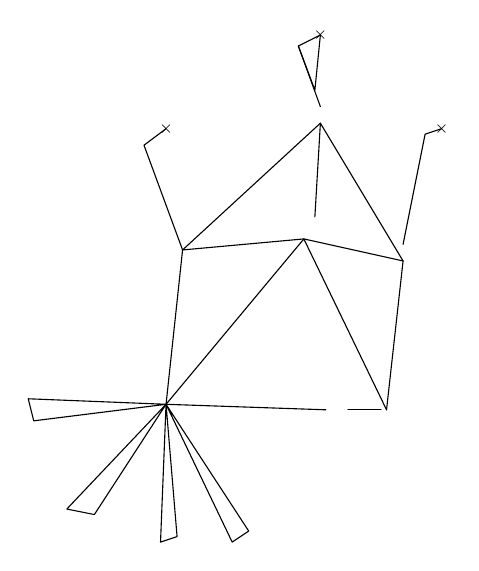
\begin{tikzpicture}[x=0.07cm,y=-0.07cm,line cap=round,line join=round,line width=.4pt]
\draw (25,67) -- (28,39) -- (53,16) -- (68,41) -- (65,68);
\draw (25,67) -- (50,37) -- (65,68);
\draw (28,39) -- (50,37) -- (68,41);
\draw (53,16) -- (52,33);
\draw (25,67) -- (54,68);
\draw (58,68) -- (64,68);
\draw (25,67) -- (0,66) -- (1,70) -- cycle;
\draw (25,67) -- (7,86) -- (12,87) -- cycle;
\draw (25,67) -- (24,92) -- (27,91) -- cycle;
\draw (25,67) -- (37,92) -- (40,90) -- cycle;
\draw (28,39) -- (21,20) -- (25,17);
\node[inner sep=.55pt,anchor=center,font=\tiny] at (25,17) {$\times$};
\draw (53,13) -- (49,2) -- (53,0);
\node[inner sep=.55pt,anchor=center,font=\tiny] at (53,0) {$\times$};
\draw (68,38) -- (72,18) -- (75,17);
\node[inner sep=.55pt,anchor=center,font=\tiny] at (75,17) {$\times$};
\draw (49,2) -- (52,10) -- (53,0);
\end{tikzpicture}%
}}
\end{tikzcd}%
}

\diagram{%
\begin{tikzcd}[ampersand replacement=\&,column sep=0pt,row sep=0pt]
|[inner sep=0pt]| \vcenter{\hbox{%
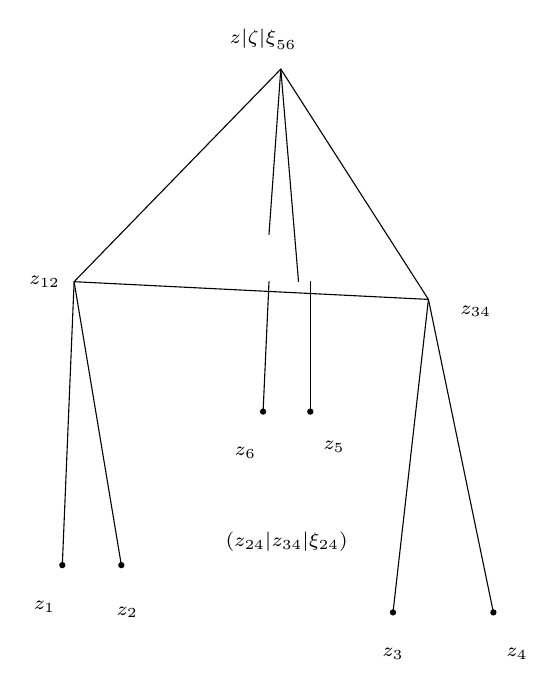
\begin{tikzpicture}[x=0.075cm,y=-0.075cm,line cap=round,line join=round,line width=.4pt]
\draw (15,36) -- (50,0) -- (75,39) -- cycle;
\draw (50,0) -- (48,28);
\draw (50,0) -- (53,36);
\draw (15,36) -- (13,84);
\draw (15,36) -- (23,84);
\fill (13,84) circle[radius=0.04cm];
\fill (23,84) circle[radius=0.04cm];
\draw (48,36) -- (47,58);
\draw (55,36) -- (55,58);
\fill (47,58) circle[radius=0.04cm];
\fill (55,58) circle[radius=0.04cm];
\draw (75,39) -- (69,92);
\draw (75,39) -- (86,92);
\fill (69,92) circle[radius=0.04cm];
\fill (86,92) circle[radius=0.04cm];
\node[inner sep=.55pt,anchor=center,font=\scriptsize] at (47,-5) {$\unsure{z|\zeta|\xi}_{56}$};
\node[inner sep=.55pt,anchor=center,font=\scriptsize] at (10,36) {$z_{12}$};
\node[inner sep=.55pt,anchor=center,font=\scriptsize] at (83,41) {$z_{34}$};
\node[inner sep=.55pt,anchor=center,font=\scriptsize] at (10,91) {$z_1$};
\node[inner sep=.55pt,anchor=center,font=\scriptsize] at (24,92) {$z_2$};
\node[inner sep=.55pt,anchor=center,font=\scriptsize] at (44,65) {$z_6$};
\node[inner sep=.55pt,anchor=center,font=\scriptsize] at (59,64) {$z_5$};
\node[inner sep=.55pt,anchor=center,font=\scriptsize] at (69,99) {$z_3$};
\node[inner sep=.55pt,anchor=center,font=\scriptsize] at (90,99) {$z_4$};
\node[inner sep=.55pt,anchor=center,font=\scriptsize] at (51,80) {$(\unsure{z_{24}|z_{34}|\xi_{24}})$};
\end{tikzpicture}%
}}
\end{tikzcd}%
}

\unsure{bicarroussel|bicaroussel|bicarrousel} épinglé

\unsure{autom} du bicarroussel d’ordre $48=2^4\cdot3$

\[
\begin{aligned}
\text{nb de \unsure{bicarousels|bicarrés|bicarrousels}} &\quad 2^3\,3^3\,5\\
&=6^3\cdot5=1080\\
&=\\
&=\underbrace{72}_{\text{\unsure{bases|racines}}}\ \underbrace{15}_{\substack{\text{nb de partitions}\\\text{d’un ens. à 6}\\\text{él. en parties}\\\text{à 2 él.}}}
\end{aligned}
\]

\diagram{%
\begin{tikzcd}[ampersand replacement=\&,column sep=0pt,row sep=0pt]
|[inner sep=0pt]| \vcenter{\hbox{%
\begin{tikzpicture}[x=0.076cm,y=-0.076cm,line cap=round,line join=round,line width=.4pt]
\draw (10,25) -- (0,59);
\draw (10,25) -- (4,71);
\draw (10,25) -- (11,60);
\draw (37,0) -- (29,28);
\draw (37,0) -- (37,37);
\draw (37,0) -- (46,35);
\draw (57,28) -- (49,68);
\draw (57,28) -- (57,78);
\draw (57,28) -- (66,68);
\draw (0,59) -- (4,62) -- (8,60) -- (11,61);
\node[inner sep=.55pt,anchor=center,font=\scriptsize] at (32,-10) {$z_{46}$};
\node[inner sep=.55pt,anchor=center,font=\scriptsize] at (108,-9) {$\deleted{\unsure{z_{36}}}\ z_{62}$};
\end{tikzpicture}%
}}
\end{tikzcd}%
}

\diagram{%
\begin{tikzcd}[ampersand replacement=\&,column sep=0pt,row sep=0pt]
|[inner sep=0pt]| \vcenter{\hbox{%
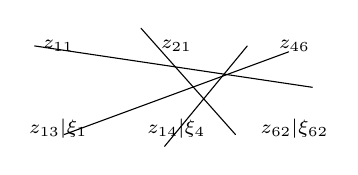
\begin{tikzpicture}[x=0.075cm,y=-0.075cm,line cap=round,line join=round,line width=.4pt]
\node[inner sep=.55pt,anchor=center,font=\scriptsize] at (0,0) {$\deleted{\unsure{z_{11}}}$};
\node[inner sep=.55pt,anchor=center,font=\scriptsize] at (20,0) {$\deleted{\unsure{z_{21}}}$};
\node[inner sep=.55pt,anchor=center,font=\scriptsize] at (40,0) {$\deleted{\unsure{z_{46}}}$};
\node[inner sep=.55pt,anchor=center,font=\scriptsize] at (0,14) {$\deleted{\unsure{z_{13}|\xi_1}}$};
\node[inner sep=.55pt,anchor=center,font=\scriptsize] at (20,14) {$\deleted{\unsure{z_{14}|\xi_4}}$};
\node[inner sep=.55pt,anchor=center,font=\scriptsize] at (40,14) {$\deleted{\unsure{z_{62}|\xi_{62}}}$};
\draw (-4,0) -- (43,7);
\draw (1,15) -- (39,1);
\draw (14,-3) -- (30,15);
\draw (18,17) -- (32,0);
\end{tikzpicture}%
}}
\end{tikzcd}%
}

\[
\begin{aligned}
&\frac{6!}{2!\,2!\,2!}\quad\cdot\binom62\binom42\frac1{3!}\\
&\qquad =\frac{15\cdot6}{6}\ =15
\end{aligned}
\]

% archive sheet number: 87
\scanpage{90}

Position relative de deux racines (ou deux bases)

Soient $r,r'$ deux racines, correspondant à des bases \deleted{$\unsure{b,b'}$} $b,b'$

\[
\begin{aligned}
r'=r^{\unsure{*|+|\prime}}&\Longleftrightarrow r.r'=-2&\Longleftrightarrow b=b'\\
r'=-r&\Longleftrightarrow r.r'=2&\Longleftrightarrow b'\ \text{associé à }b\\
r'\ \text{orth. à }r&\Longleftrightarrow rr'=0&\Longleftrightarrow\operatorname{card}(b\cap b')=\underline{1}\\
\widehat{r,r'}=60^\circ&\Longleftrightarrow rr'=-1&\Longleftrightarrow\operatorname{card}(b\cap b')=3\ \deleted{\text{\unsure{et b,b′ associés}}}\\
\widehat{r.r'}=120^\circ&\Longleftrightarrow rr'=1&\Longleftrightarrow\operatorname{card}(b\cap b')=\deleted{\unsure{1|4}}0\\
&&\quad\deleted{\text{\unsure{et b,b′ associés}}}\ \inserted{\text{et }b,b'\text{ non \underline{associés}.}}
\end{aligned}
\]

Pour une racine $r$ donnée, il y a

\[
\begin{aligned}
1&\ \text{racine égale à }r,\ \text{soit }r\\
1&\ \text{racine opposée à }r,\ \text{soit }-r\\
30&\ \text{racines orthogonales à }r\\
20&\ \deleted{\text{\unsure{racines}}}\ \text{faisant un angle de }60^\circ\ \text{avec }r\\
20&\quad\rule{6em}{.3pt}\quad120^\circ\quad\rule{1.5em}{.3pt}\quad r
\end{aligned}
\]

\[
\begin{aligned}
\deleted{\text{\unsure{couples}}}\text{\unsure{paires|couples} de racines égales}&\quad72\\
\rule{5em}{.3pt}\ \text{opposées}&\quad72/2=36\\
\deleted{\text{\unsure{couples}}}\text{\unsure{paires|couples} de racines orthogonales}&\quad72\cdot15=1080\\
\deleted{\text{\unsure{couples}}}\text{\unsure{paires|couples} de racines à }60^\circ&\quad72\cdot10=720\\
\rule{4em}{.3pt}\quad120^\circ&\quad\underline{\underline{72\cdot10=720}}
\end{aligned}
\]

plans de \inserted{paires de} racines non orthogonales (= plans spéciaux) \quad $720:6=120\deleted{\unsure{=2^3\cdot3}}$

% archive sheet number: 89
\scanpage{91}

\deleted{%
\[
\begin{aligned}
&\deleted{x-w}&&r_0-2r_1-r_2+r_6\\
&\deleted{x-s_r(x)}\\
&s_r(x):x+(r,x)r&&r_1+2r_2+3r_3+2r_4+r_5+3r_6\\
&s_r(x)-x=(r,x)r\\
&(r,x)\in\{0,1,-1\}&&\alpha_1\\
&(\deleted{x-y}\quad s_rx-x=\\
&\deleted{x-wx=}\\
&wx=x+\rho\qquad \rho\ \text{\unsure{racine|vecteur}}\\
&s_rwx=s_rx+s_r\rho=x+\underbrace{(x,r)}_{\varepsilon}r+s_r\rho\\
&a)\ (x,r)=0\quad\text{i.e. }s_rx=x\quad\text{\unsure{on gagne}}\\
&b)\ (x,r)=1\\
&\quad\text{\unsure{on trouve}}\quad s_rwx-x=s_r\rho+r
\end{aligned}
\]
}

\[
\begin{aligned}
3\unsure{z|\zeta|\xi}_i-\lambda&=3z_i-3\eta+\zeta=-3\eta+\sum_{\alpha\ne i}z_\alpha+4z_i\\
&\deleted{\unsure{3}}z_i-\lambda
\end{aligned}
\]

\[
\widetilde z_i=3z_i-\lambda
=\underbrace{3(z_i-z_1)}_{-3(r_1+r_2+\cdots+r_{i-1})}
+\underbrace{(3z_1-\eta)}_{-r_6+2r_1+r_2}
+\underbrace{\eta-\lambda}_{-r_0}
\]

\[
\begin{aligned}
-\widetilde z_i={}&\deleted{\unsure{(r_0+2r_1+r_2)}}\ \deleted{\unsure{2r_1+2r_2}}\
+3(r_1+\cdots+r_{i-1})\deleted{\unsure{+2r_1}}-r_2+\deleted{\unsure{r_6}}r_6\\
&+\deleted{\unsure{r_0}}r_1+2r_2+3r_3+2r_4+r_5+2r_6
\end{aligned}
\]

\[
\begin{aligned}
-\widetilde z_1^{\deleted{\unsure{-}}}&=-r_1+\unsure{1|4|2}r_2+3r_3+2r_4+r_5\deleted{+r_6}+3r_6\\
-\widetilde z_{2}&=2r_1+\unsure{1|4|2}r_2+3r_3+2r_4+r_5+3r_6\\
-\widetilde z_3&=2r_1+\unsure{4|9}r_2+3r_3+2r_4+r_5+3r_6\\
-\widetilde z_4&=2r_1+4r_2+6r_3+2r_4+r_5+3r_6\\
-\widetilde z_{\unsure{5|6}}&=2r_1+\unsure{4|9}r_2+6r_3+5r_4+r_5+3r_6\\
-\widetilde z_6&=2r_1+\unsure{4|9}r_2+6r_3+5r_4+4r_5+3r_6
\end{aligned}
\]

\[
\deleted{-\widetilde\eta=\unsure{3}(r_1+r_2+r_3)+6r_4+3r_5+9r_6}
\]

\[
\begin{aligned}
\widetilde\eta&=3\eta-3\lambda=-3(\lambda-\eta)=-3r_0.\\
-\widetilde\eta&=+3r_1+6r_2+9r_3+6r_4+3r_5+6r_6
\end{aligned}
\]

% archive sheet number: 90
\scanpage{92}

\deleted{%

\[
\begin{aligned}
a+3b&=-2\\3a+\unsure{3|1|9}b&=0\\
\deleted{2a=}\qquad a&=-b/3\\
\unsure{8}a&=2\qquad a=\tfrac14\\
&\qquad b=\\
a+\unsure{8|3}b&=-1
\end{aligned}
\]

\[
\begin{aligned}
&a+3b+\\
&a+3b+2,\ a+3b+3\\
&a+3b,\ a+3b+1\\
&a+3b^{\unsure{\prime\prime|\prime}}-3,\ a+3b^{\prime}-2
\end{aligned}
\]

\[
\begin{aligned}
&2\quad-1\\
&x=a\eta+b\zeta+\unsure{z|\zeta|\xi}_i\qquad
\left\{\begin{aligned}a+3b&=-1\\3a+b&=0\end{aligned}\right\}
\quad x=b(\overline{\zeta-\tfrac{\eta}{3}})+z_i\\
&\deleted{\unsure{=2a+6b=}}\\
&x=a\eta+b'\zeta-z_i\\
&\underline{3a+6b=0}\qquad a=2b\\
&\deleted{3a+6b=}
\end{aligned}
\]

\[
\begin{aligned}
\text{\textcircled{1}}\quad x&=a\eta+b\zeta+z_i\\
\alpha)\quad a+3b&=-1\quad \text{i.e. }\boxed{b=-1,\ a=2}
   \quad 2\eta-\zeta+z_i=\boxed{z'_i}\\
\beta)\quad a+3b&=0\quad \text{i.e. }\ b=0,\ a=0\qquad \deleted{\unsure{=2a}}\quad\boxed{z_i}\\
3a+6b&=0\\a+2b&=0\\a&=-2b
\end{aligned}
\]

\[
\begin{aligned}
\text{\textcircled{2}}\quad x&=a\eta+b\zeta-z_i\\
\text{posons}\quad x'&=2\lambda_0-x=\deleted{\unsure{\tfrac23\lambda}}2\eta-\tfrac23\zeta-a\eta-b\zeta+z_i\\
\lambda_0&=\eta-\tfrac{\zeta}{3}\qquad
=\underbrace{(2-a)}_{a'}\eta+\underbrace{\left(-\tfrac23-b\right)}_{b'}\zeta+z_i
\end{aligned}
\]
on est dans le cas précédent

\[
\begin{aligned}
\text{\textcircled{3}}\quad x&=a\eta+b\zeta-z_i-z_j\qquad a+3b=1\\
3a+6b&=3\qquad a+2b=1\qquad
\boxed{\begin{aligned}b&=0\\a&=1\end{aligned}}\qquad\boxed{z_{ij}}\\
&a=1-2b
\end{aligned}
\]

\[
\text{\textcircled{4}}\qquad x=a\eta+b\zeta+z_i+z_j\qquad\text{est ramené au cas \unsure{préc. par}}
\]
\[
\delta\quad\unsure{-|\mapsto|\sim}\quad-(\delta-\lambda_0)+\lambda_0=2\lambda_0-\delta=\tfrac23\lambda-\delta=\delta'
\]

\[
\begin{aligned}
r_1&\longrightarrow-r_5\\r_2&\mathrel{-}-r_4\\r_3&\mathrel{-}-r_3\\
r_4&\unsure{\leftarrow|-|\longmapsto}-r_2\\r_5&\mathrel{-}-r_1\\ \noalign{\smallskip\hrule\smallskip}
r_6&\longrightarrow r_{456}=r_6+\\
\unsure{''r_{123}|r_{12}}&\quad 3(r_1+r_2+r_3)\\
&\qquad+2r_4+r_5
\end{aligned}
\]

\[
\begin{aligned}
r_{ijk}&=\eta\overset{\frac23}{-}z_i\ z_j-z_k\\
\eta-z_3-z_5-z_{\unsure{r|6}}&=\eta-z_1-z_2-z_3+
 (z_1-z_4)+(z_2-z_5)+\\
&\qquad +z_3-z_{\unsure{6}}
\end{aligned}
\]

}% end of diagonal cancellation
% archive sheet number: 91
\scanpage{93}

\deleted{%
\[
\begin{aligned}
\unsure{z|\zeta|\xi}'_i&=\deleted{\unsure{3\eta}}r_0+z_i\ \deleted{\unsure{=}}\\
\widetilde z'_i&=\widetilde r_0+\widetilde z_i=3r_0+\widetilde z_i\ \unsure{\Rightarrow}\quad \unsure{\zeta\longmapsto\lambda|\{1\longrightarrow\}\ \lambda|\{i\mapsto{}\}\ \lambda}\\
-\widetilde z'_i&=\unsure{-\widetilde z_i-\widetilde r_0=}
\end{aligned}
\]
}

\[
\begin{aligned}
3z'_i&=\unsure{z_i|3z_i|\xi_i}+3r_0\\
\widetilde{3z'_i}&=\widetilde{3z_i}+3r_0\\
z'_i-z_i&=r_0\qquad=3\widetilde z_i-\widetilde\eta\\
-\unsure{3z'_i|3\widetilde{\xi}'_i}&=-\widetilde z_i+\widetilde\eta
\end{aligned}
\]

\[
\begin{aligned}
-\widetilde z'_i&=-\widetilde z_i-3r_0
=-\widetilde z_i-3(r_1+r_2+r_3)-6r_4-3r_5-6r_6\\
&=-\widetilde z_i-\widetilde\eta\\
&\deleted{\unsure{-3r}}
\end{aligned}
\]

\[
\begin{aligned}
z_{ij}&=\eta-z_i-z_j\\
\widetilde z_{ij}&=\widetilde\eta-\widetilde z_i-\widetilde z_j
=(-\widetilde z_i)+(-\widetilde z_j)-(-\widetilde\eta)\\
&\deleted{-\widetilde z_{ij}=\widetilde z_i+\widetilde z_j+\unsure{6\widetilde\eta}}
\end{aligned}
\]

\unsure{pté|parti}

\[
\begin{array}{l@{\qquad}l@{\qquad}r}
&&-\widetilde\delta=-w(-\widetilde\delta)\\
\deleted{1,4,-8,-5,-4,-1}&\deleted{-8,-5,-4,-1,1,4}&6\\
\deleted{2,5,-7,-4,-5,-2}&\deleted{-7,-5,-4,-2,2,5}&6\\
\deleted{3,6,-6,-3,-3,0}&\deleted{-6,-3,0,3,6}&5\\
\deleted{2,5,-4,-1,-2,1}&\deleted{-4,-2,-1,1,2,5}&6\\
\deleted{1,4,-2,1,-1,2}&\deleted{-2,-1,1,2,4}&5\\
\deleted{3,-3,-3}&\deleted{-3,3}&2
\end{array}
\]

\[
\begin{aligned}
\widetilde\delta&=\deleted{\unsure{w}}-w(\widetilde\delta)\\
&=-\widetilde{w(\delta)}=-\widetilde{\delta'}\\
\widetilde{\delta+\delta'}&=0\\
\#\{\delta+\delta'\}&=27=
\end{aligned}
\]

\diagram{$\begin{array}{r|r|r|r|r|r|r}
&r_1&r_2&r_3&r_{\unsure{4|2}}&r_5&r_6\\ \hline
-\widetilde z_{1}&-1&1&3&2&1&3\\
-\widetilde z_{2}&2&1&3&2&1&3\\
-\widetilde z_{3}&2&4&3&2&1&3\\
-\widetilde z_{4}&2&4&6&2&1&3\\
-\widetilde z_{5}&2&4&5&5&1&3\\
-\widetilde z_{6}&2&4&6&5&4&3\\ \hline
-\widetilde z_{1}'&2&7&12&8&4&9\\
-\widetilde z_{2}'&5&7&12&8&4&9\\
-\widetilde z_{3}'&5&10&12&8&4&9\\
-\widetilde z_{4}'&5&10&15&8&4&9\\
-\widetilde z_{5}'&5&10&15&11&7&9\\
-\widetilde z_{6}'&5&10&15&11&10&9\\ \hline
&-2&-4&-3&-2&-2&0\\
&1&-1&0&1&1&0\\
\end{array}$}

\[
\begin{aligned}
\widetilde\delta&=-w(\widetilde\delta)\\
&=-\widetilde{w(\delta)}\\
&=-\widetilde{\delta'}\\
\widetilde{\delta+\delta'}&=0
\end{aligned}
\]

\[
\begin{aligned}
&-2,-1,1,2,5\\&-2,1,4,7,10
\end{aligned}
\]

% archive sheet number: 92
\scanpage{96}

$R\subset E$ syst. de racines ($E$ $\mathbb R$-vectoriel engendré par $R$)

produit scalaire invariant tel que $(r,r)=2$ $\forall r\in R$ (racines ttes de même longueur)

\[
\begin{aligned}
\unsure{\mathscr S|\mathscr G|\mathfrak S}&=\{x\in E^*\mid (x,r)\deleted{\tfrac{2}{(r,r)}}\in\{-1,0,1\}\ \forall r\in R\}\\
\mathscr S_0&=\{x\in E^*\mid wx-x\in R\quad\forall w\in W\ \text{t.q. }wx\ne x\}
\end{aligned}
\]

où $E^*=E-\{0\}$\\ où \deleted{$E$}$W={}$groupe de Weyl.

$\mathscr S_0\subset\mathscr S$, car $\mathscr S_0\subset E^*$, et \inserted{$x\in\mathscr S_0\Rightarrow$} $s_rx-x=-2\frac{\langle x,r\rangle}{(r,r)}r\in R$, donc si $s_rx\ne x$ i.e. $\langle x,r\rangle\ne0$, on a $-(x,r)\in\frac{(r,r)}2\{\pm1\}$, donc \deleted{\unsure{on}} tjrs \unsure{un|on|cas} $(x,r)\in\{-1,0,+1\}$.

\deleted{\unsure{Card $\mathscr S$}}

$\operatorname{Card}\mathscr S\leq3^r-1$ donc $\mathscr S$ et a fortiori $\mathscr S_0$ fini.

$\mathscr S,\mathscr S_0$ stables par $W$ et même par $\widehat W=\operatorname{Aut}(E,R)$, et $W$ a un nb fini d’orbites dans $\mathscr S$ et a fortiori dans $\mathscr S_0$.

Cas $(A_r)$

\[
\begin{aligned}
E&=\mathbb R^{r+1},\ E=\{(x_1,\ldots x_{r+1})\mid\sum_1^{r+1}x_i=0\}\\
R&=\{\alpha_{ij}=\varepsilon_i-\varepsilon_j\mid i\ne j,\ 1\leq i,j\leq r+1\}\\
\operatorname{Card} R&=r(r+1)
\end{aligned}
\]

produit scalaire induit par $(\xi,\eta)=\sum_1^{r+1}\xi_i\eta_i$ sur $\mathbb R^{r+1}$ \deleted{\unsure{est fourni par}}

\[
\begin{aligned}
&\xi_{\unsure{1|0}}\ldots\xi_r\qquad\sum\xi_i=0\\
&\underbrace{\xi_{1}=\cdots=\xi_{r_1}}_{\alpha_1}\quad
\underset{<}{\phantom{a}}\underbrace{\xi_{r_1+1}=\cdots=\xi_{r_1+r_2}}_{\alpha_2}
\quad\ldots,\quad
\underbrace{\xi_{r_1+r_2+\cdots+r_{s-1}+1}=\xi_{\underbrace{r_1+r_2+\cdots+r_s}_{r+1}}}_{\alpha_s}
\end{aligned}
\]

\[
\begin{aligned}
\left\{\begin{aligned}
r_1\alpha_1+r_2\alpha_2\ \cdots+r_s\alpha_s&=0\\
r_1+r_2\ \cdots+r_s&=r+1
\end{aligned}\right.&\qquad
\begin{aligned}\alpha_1&<\alpha_2\ \cdots<\alpha_s\\r_1,r_2&\ \cdots r_s\geq1\end{aligned}\\
\alpha_i-\alpha_j\in\{\pm1\}\quad&\forall i,j\quad\ne
\end{aligned}
\]

Soit \deleted{\illegible{2}} $s=1$, \deleted{\unsure{on}} $r_1=r+1$, $r_1\alpha_1=(r+1)\alpha_1=0$, $\alpha_1=0$ \unsure{abs.|et} donc $\xi=0$, absurde.

Soit $s=2$.

\[
\begin{aligned}
\alpha_2=\alpha_1+1\qquad&
\left\{\begin{aligned}
r_1\alpha_1+r_2\alpha_2&=0\\r_1+r_2&=r+1\\\alpha_2&=\alpha_1+1
\end{aligned}\right.
\ \Longrightarrow
\begin{aligned}
(r_1+r_2)\alpha_1+r_2&=0\\
\text{i.e. }(r+1)\alpha_1+r_2&=0\\
\text{i.e. }\alpha_1&=\frac{-r_2}{r+1}
\end{aligned}\\
\deleted{\text{Il y a }r+}\qquad&
\alpha_1=\frac{-r_2}{r+1},\ \alpha_2=\frac{r_1}{r+1}\qquad r_1+r_2=r+1
\end{aligned}
\]

il y a $r+1$ classes de tels élément, suivant la valeur de $1\leq r_1\leq r+1$

% archive sheet number: 97
\scanpage{97}

\[
\underbrace{-\frac{r_2}{r+1},\ldots,-\frac{r_2}{r+1}}_{r_1},
\underbrace{\frac{r_1}{r+1},\ldots,\frac{r_1}{r+1}}_{r_2}
\qquad
[1,r+1]=\underbrace{[1,r_1]}_{I_1}\cup\underbrace{[r_1+1,r+1]}_{I_2}
\]
\[-\frac{r_1}{r+1}\quad-\frac{r_2}{r+1}\qquad\pm1\qquad \sigma^{\unsure{-1}}I_1,\ \sigma I_2\]

\[
\begin{aligned}
\xi&\qquad\alpha_1\text{ sur }I_1,\ \alpha_2\text{ sur }I_2\\
\sigma.\xi&=\xi\circ\sigma^{-1}\qquad\alpha_1\text{ sur }\sigma I_1,\alpha_2\text{ sur }\sigma I_2\\
\xi-\sigma\xi&\qquad 0\text{ sur }(I_1\cap\sigma I_1)\cup(I_2\cap\sigma I_2)\\
&\qquad-1\text{ sur }I_1\cap\sigma I_2\\
&\qquad 1\text{ sur }I_2\cap\sigma I_1
\end{aligned}
\]

On veut, $\forall\sigma$ tel que $\sigma I_1\ne I_1$ \inserted{et $\sigma I_2\ne I_2$}, \deleted{\unsure{que}} \inserted{i.e. $\sigma I_2\cap I_1\ne\varnothing$} i.e. $\sigma I_1\cap I_2\ne\varnothing$

\deleted{$I_1\cap\sigma I_2$}

\[
\begin{aligned}
\operatorname{card}(I_1\cap\sigma I_2)&=1\ \to\ \text{c’est possible \inserted{(pour tout $\sigma$)} ssi }\operatorname{card}I_1\leq1\text{ ou card }I_2\leq1\\
\operatorname{card}(I_2\cap\sigma I_1)&=1\qquad\rule{1em}{.3pt}\quad\rule{1em}{.3pt}
\end{aligned}
\]

\deleted{Donc} OK ssi $r_1=1$ ou $r_2=1$

\[
\begin{aligned}
&-\frac1{r+1},\underbrace{\frac r{r+1},\ldots,\frac r{r+1}}_r\\
&\underbrace{-\frac r{r+1},\deleted{\unsure{\tfrac1{r+1}}}\ldots,-\frac r{r+1}}_r,\frac1{r+1}
\end{aligned}
\]

2 orbites \inserted{(si $r\geq2$)} \unsure{pour|sous} $W$, qui sont \deleted{\unsure{conjuguées par}} \inserted{transformées} l’une de l’autre par \unsure{l’élém|l’élément} \deleted{\unsure{non triv}} de $\unsure{\Gamma|E}=\widehat W/W$ i.e. par la symétrie !

$\text{\textcircled{$B_r$}}\qquad V=E=\mathbb R^r$

\[
\begin{aligned}
R&=\{\pm\varepsilon_i\ (1\leq i\leq r)\quad\pm\varepsilon_i\pm\varepsilon_j\ (1\leq i<j\leq r)\}\\
&2r+4\frac{r(r-1)}2=2r+2r(r-1)=2r^2
\end{aligned}
\]

\[
2r+1\quad
\begin{pmatrix}\lambda&&a_{ij}\\-a_{ij}&\ddots&\\&&0\end{pmatrix}
\qquad
\begin{pmatrix}\lambda_1\\&\lambda_1^{-1}\\&&\ddots\\&&&\lambda_r\\&&&&\lambda_r^{-1}\\&&&&&1\end{pmatrix}
\]

Produit scalaire habituel, longueurs 1 et 2

\[
\begin{aligned}
\xi&=(\xi_1,\xi_2\ldots\xi_r)\quad\unsure{\forall\xi|\deleted{\xi_i}}\quad0\leq\xi_1\leq\xi_2\leq\ldots\leq\xi_r\\
&\underbrace{\xi_1\ldots\xi_{r_1}}_{\alpha_1}\quad\underbrace{\xi_{r_1+1}\ldots\xi_{r_1+r_2}}_{\alpha_2}\ \ldots\
\underbrace{\xi_{r_1+\cdots+r_{s-1}+1}\ldots\xi_{r_1+\cdots+r_s=r}}_{\alpha_s}\\
(\xi,\varepsilon_i)&\in 2\cdot\{-1,0,1\}\qquad\text{i.e. }\boxed{\xi_i\text{ égale }0\text{ ou }2}\\
(\xi,\varepsilon_i\pm\varepsilon_j)&=\xi_i\pm\xi_j\in\{1,0,-1\}\\
&\deleted{\unsure{\xi}}\quad\alpha_i+\alpha_j=1\quad\deleted{\unsure{\text{i.e.}}}\\
&\phantom{x}\quad\alpha_i-\alpha_j=-1\qquad\text{si }1\leq i<j\leq s\\
&\hspace{12em}\unsure{\forall}
\end{aligned}
\]

\deleted{\unsure{bien seule|Une seule} donc} impossible, donc $s=1$

\[\xi=(2,2,\ldots,2)\qquad\unsure{\mathscr S|\mathscr G|\mathfrak S}=\varnothing\]

$\text{\textcircled{$C_{\unsure{r|6}}$}}\qquad E=\mathbb R^r$

\[
R=\{\pm2\varepsilon_i\ \inserted{(1\leq i\leq r)},\ \pm\varepsilon_i+\varepsilon_j\}\ (1\leq i\leq j\leq r))
\]

\deleted{\unsure{ce}}\qquad $\deleted{\unsure{\xi_i\in}}$

\[
\begin{aligned}
(\xi_i)_{1\leq i\leq r}&\qquad \xi_i\in\tfrac24\{-1,0,+1\}=\{\\
0\leq\xi_1&\leq\ldots\leq\xi_r\qquad\text{i.e. }\xi_1\in\{0,\tfrac12\}\\
\pm\xi_i\pm\xi_j&\in\{-1,0,+1\}\\
\deleted{\unsure{\theta}}&(\tfrac12,\tfrac12\ldots,\tfrac12)\qquad\deleted{r\geq3}\quad r\geq3\\
\mathscr S&=\deleted{\unsure{\tfrac12\{\varepsilon_1,\varepsilon_2,\ldots\}}}\ \deleted{\unsure{\tfrac12}}\{\pm\tfrac12\}^r\qquad\unsure{=}\\
\mathscr S_0&=\varnothing
\end{aligned}
\]

$\text{\textcircled{$D_r$}}\qquad E=\mathbb R^r$

\[
\begin{aligned}
R&=\{\pm\varepsilon_i\pm\varepsilon_j\quad1\leq i<j\leq r\}\\
&\deleted{\unsure{\xi}}\quad \xi_1\ldots\xi_r\\
&\xi_1\leq\underset{\geq0}{\xi_2}\ldots\leq\xi_r\quad \pm\xi_i\pm\xi_j\in\{-1,0,1\}
\end{aligned}
\]

au plus \deleted{deux} valeurs distinctes des $\xi_i$, différant de 1, soit $\alpha$ et $\alpha+1$, \inserted{mais \deleted{\unsure{on|$\alpha+$}} $2\alpha+1\in\{-1,0,1\}$ i.e.} ou bien ttes les valeurs égales, égales : $\pm\frac12$

\[
\begin{aligned}
\deleted{2\alpha+1=0}&\quad\alpha=-\tfrac12\quad\alpha+1=\tfrac12
&-\tfrac12,\underbrace{\tfrac12,\tfrac12\ldots\tfrac12}_{r-1}\\
2\alpha+1=1&,\ \alpha=0&(\underbrace{0,\ldots0}_{\unsure{r-1|r+1}},\underbrace{1}_{r_2=1})\ \deleted{\unsure{1-}}\ \to r\\
2\alpha+1=-1&,\ \alpha=-1&(-1,\underbrace{0,\ldots,0}_{r-1})
\end{aligned}
\]
\deleted{\unsure{au facteur}}\quad à conj. près $(r_2=1)$

\[
\begin{aligned}
&\bigl(\tfrac12(\unsure{\varepsilon|\pm})_i\bigr)\qquad
\deleted{\unsure{\{\pm1\}}}\quad\prod(\unsure{\varepsilon})_i=1
\ \Big\}\cdot(\tfrac12,\tfrac12,\ldots,\tfrac12)\\
&\ldots\qquad\qquad\rule{1em}{.3pt}\qquad\prod(\unsure{\varepsilon})_i=-1\\
&\deleted{\unsure{\varepsilon_i}}\{\pm\varepsilon_i\}
\end{aligned}
\]

\deleted{il y a \unsure{trois}} $\mathscr S$ a trois orbites\\ $\mathscr S_0=\varnothing$ \deleted{\unsure{et a une orbite}}

% archive sheet number: 98
\scanpage{98}

\[
\unsure{\mathscr S|\mathscr G|\mathfrak S}'_0=\{x\in E\mid w\in W,\ w(\mathbb R x)\ne\mathbb R x\Longrightarrow wx-x\in R\}
\]

\[
\begin{aligned}
x\in\mathscr S'_0,\quad r\in R\qquad&s_rx-x=2\frac{(x,r)}{(r,r)}r\\
s_r(\mathbb R x)&=(\mathbb R x)\Longleftrightarrow s_rx=x\text{ ou }s_rx=-x\\
&\Longleftrightarrow (x,r)=0\text{ ou }x\in\mathbb R r
\end{aligned}
\]

\[(x,r)\ne0\text{ et }x\notin\mathbb R r\Longrightarrow\underbrace{2\frac{(x,r)}{(r,r)}}_{\unsure{n_{x,r}|n_{x r}}}=\pm1\]

\deleted{$(x,r)$ \unsure{de|donc}}\quad .

\diagram{%
\begin{tikzcd}[ampersand replacement=\&,column sep=small,row sep=0pt]
 \mathscr S_0^{\unsure{\prime\prime|\prime}}\&\subset\&\mathscr S'\&
 =\{x\in E\mid \forall r\in R\cap\complement\mathbb R x,\ \text{on a }(x,r)\in\tfrac{(r,r)}2\{-1,0,+1\}\}\\
 \cup\&\&\cup\\
 \mathscr S_0\&\subset\&\mathscr S
\end{tikzcd}%
}

\[
\begin{aligned}
\mathscr S'&=\mathscr S\cup\{\lambda s\mid s\in R,\lambda\in\mathbb R^{++},\
 (\lambda s,\unsure{r})\in\tfrac{(r,r)}2\{-1,0,1\}\\
&\hspace{16em}\forall r\in R-\{s,-s\}\}\\
&\text{i.e.}\qquad \forall r\in R-\{s,-s\}\unsure{-|\ne}(R\cap s^\perp)\\
&\deleted{\text{i.e. }\lambda\in\tfrac{(r,r)}{2(s,r)}}\qquad
 \lambda\in\tfrac{(r,r)}{2(s,r)}\{-1,0,1\}\\
&\text{i.e. }\lambda=\pm\tfrac{(r,r)}{2(s,r)}\qquad
 \text{i.e. }\tfrac1\lambda=\pm\tfrac{2(s,r)}{(r,r)}=\pm n(s,r)
\end{aligned}
\]

un tel $\lambda$ existe (il est unique au signe près), pour $s$ donné, ssi les quantités $\left|\frac{(s,r)}{(r,r)}\right|$, pour $r$ racine non orthogonale ni prop. à $s$, sont égales, i.e. ssi il n’y a qu’un seul angle de droites possible (savoir $\frac\pi3$, \inserted{d’où $n(s,r)=\pm1$, d’où $\lambda=\unsure{s|1|\pm1}$}) pour des racines distinctes non orth. C’est le cas ssi ttes les racines sont de $=$ longueur, i.e. les types $A_n$, $D_n$, $E_i$ $(6\leq i\leq8)$.

% archive sheet number: 99
\scanpage{99}

\[
\unsure{\mathscr S|\mathscr G|\mathfrak S}_{\unsure{\bullet|0}}^{\deleted{\unsure{*}}\prime}
=\left\{\begin{aligned}
&\mathscr S_{\unsure{\bullet|0}}\quad\text{si ttes les racines pas de $=$ longueur}\\
&\mathscr S_{\unsure{\bullet|0}}\cup R\quad\text{si \deleted{\unsure{non}} ttes les racines de $=$ long.}
\end{aligned}\right.
\]

\deleted{%
\[
\begin{aligned}
\mathscr S'_0&=\left\{\begin{aligned}&\mathscr S_0\text{ si ttes les}\\&\unsure{\subset}\mathscr S_0\text{ si ttes les racines pas de $=$ longueur}\end{aligned}\right.\\
\mathscr S'_0&=\\
\mathscr S'_0&\cap\mathscr S
\end{aligned}
\]
}

\uline{Cas de} $A_r$ $(r\geq2)\qquad \mathscr S'=\mathscr S\cup R$

\[
r+2\ \text{classes}\quad
\deleted{\underbrace{\unsure{-\tfrac{r_2}{r+1},\ldots,-\tfrac{r_2}{r+1}}}_{\unsure{\cdot}}}
\left\{\begin{aligned}
&-\tfrac{r_2}{r+1}(e_1+\cdots+e_{r_1})+\tfrac{r_1}{r+1}(e_{r_1+1}+\cdots+e_{r_1+r_2})\\
&1\leq r_2\leq\unsure{r+1|r-1}\\
&e_1-e_2
\end{aligned}\right.
\]

\diagram{%
\begin{tikzcd}[ampersand replacement=\&,column sep=0pt,row sep=0pt]
|[inner sep=0pt]| \vcenter{\hbox{%
\begin{tikzpicture}[x=0.065cm,y=-0.065cm,line cap=round,line join=round,line width=.4pt]
\draw (0,6) -- (28,6) -- (61,6);
\draw (0,3) -- (0,9);
\draw (28,3) -- (28,9);
\draw (61,3) -- (61,9);
\node[inner sep=.55pt,anchor=south,font=\scriptsize] at (14,4) {$r_1$};
\node[inner sep=.55pt,anchor=south,font=\scriptsize] at (45,4) {$r_2$};
\end{tikzpicture}%
}}
\end{tikzcd}%
}

\[
\mathscr S'_0=\left\{\begin{aligned}
&\mathscr S_0\text{ si }r\ne3\quad\text{i.e. }r+1\ne4\\
&\unsure{\mathscr S_0|\mathfrak S_0}\cup W.(-\tfrac12,-\tfrac12,\tfrac12,\tfrac12)
\end{aligned}\right.
\]

% archive sheet number: 100
\scanpage{101}

\[\begin{aligned}&\quad G\\ &N_1\quad N_2\quad N_3\end{aligned}\]

\diagram{%
\begin{tikzcd}[ampersand replacement=\&,row sep=small,column sep=small]
 \&G/N_1\\
 \&G\arrow[u]\arrow[dr]\arrow[dl,dash]\\
 G/N_3\&\&G/N_2
\end{tikzcd}%
}

\[
\begin{aligned}
&\unsure{\therefore}\\
&N_1\cap N_2=\{e\}\\
&\forall x_1\in G,\ x_2\in G\\
&\exists x\in G,\quad x\in x_1N_1\cap x_2N_2\\
&\text{i.e. }\left\{\begin{aligned}x_1^{-1}x&\in N_1\\x_2^{-1}x&\in N_2\end{aligned}\right.
\end{aligned}
\]

\[
\begin{aligned}
N_1\times N_2&\longrightarrow G\\
(x_1,x_2)&\longrightarrow x_1x_2\\
x_1x_2&=y_1y_2\\
(y_1^{-1}x_1)&=(y_2x_2^{-1})\in N_1\cap N_2=\{e\}\\
x_1&=y_1,\ x_2=y_2
\end{aligned}
\]

\[
\begin{aligned}
&\deleted{N_1N}\\
&N_1.N_2=G\quad\Longleftrightarrow\quad N_2N_1=G\\
&\unsure{a_r}\qquad \deleted{x_1\in G}\\
&a_1b_2=x_1\\&d_2c_1=x_2\\&a_{1} \quad a
\end{aligned}
\]

\diagram{%
\begin{tikzcd}[ampersand replacement=\&,column sep=small,row sep=small]
 \&N_1\overset{\sim}{\to}G/N_2\&x\\
 N_1\times N_2\overset{\sim}{\to}G\arrow[ur]\arrow[r]\arrow[dr]\&{}\&\\
 \deleted{(x_1,x_2)\to x_1x_2}\arrow[uurr,bend left=16]\&N_2\simeq G/N_1
\end{tikzcd}%
}

\diagram{%
\begin{tikzcd}[ampersand replacement=\&,row sep=small,column sep=small]
 x=a_1a_2\arrow[r]\&a_1\in N_1\simeq G/N_2\&a_1=x_1\\
 {}=b_2b_1\arrow[dr]\&\deleted{\unsure{a_1x_2|x_1x_2}}\arrow[ur]\arrow[dr]\&\\
 \&\deleted{\unsure{b_2\in}}\ N_2\&{}\simeq G/N_1
\end{tikzcd}%
}

\[
\begin{aligned}
x&=x_1a_2\\x^{\unsure{\prime|\prime\prime}}&=x'_2b_1\\
x_1a_2&=x_2b_1\\
x_2^{-1}x_1&=b_1a_2^{-1}=b_1a'_2
\end{aligned}
\]

\[
\left\{\begin{aligned}
N_2\cap N_3&=N_3\cap N_1=N_1\cap N_2=\{e\}\\
N_2N_3&=N_3.N_1=N_1.N_2=G
\end{aligned}\right.
\]
\[G\simeq N_2\mathbin{\underset{1/2}{.}}N_1\simeq N_3\mathbin{\underset{1/2}{.}}N_1\]

\margin{\deleted{\unsure{$G/$}}\\ $N_1$ invariant\\ $G/N_1\simeq\unsure{V|\forall}$\\ $N_2\qquad N_3$}

% archive sheet number: 102
\scanpage{102}

\diagram{\begin{tikzcd}[ampersand replacement=\&,row sep=small]
 N_{\deleted{\unsure{1|2}}\unsure{2|1}}\times N_{\deleted{\unsure{2|3}}3}\\
 N_1\arrow[u]
\end{tikzcd}}

\diagram{\begin{tikzcd}[ampersand replacement=\&,row sep=small]
 G\times G=\Gamma\\G\arrow[u,hook]
\end{tikzcd}}

\[
\begin{aligned}
&G\times e=N_2\quad e\times G=N_3\quad\delta G=N_1\\
&\deleted{(g,h)=}\\
&(g,e)\quad(e,h)\\
&\qquad(k,k)
\end{aligned}
\]

\[
\begin{aligned}
&(g,h)(k,k)(g,h)^{-1}\\
&=gkg^{-1},hkh^{-1}
\end{aligned}
\]

\diagram{\begin{tikzcd}[ampersand replacement=\&,row sep=small,column sep=small]
 \&G\\
 \&G\times G\arrow[u,"\mathrm{pr}_2"]\arrow[r,"\mathrm{pr}_3"]\arrow[dl,"\mathrm{pr}_1"']\arrow[ddl,bend left=45,"\delta(g{,}h)=gh^{-1}"]\&G\\
 G\times G/\delta G\\
 G\arrow[u,"\unsure{\simeq|21}",phantom]
\end{tikzcd}}

\[
\begin{aligned}
(g,h)&\to gh^{-1}\deleted{\unsure{\ne}}\\
gh^{-1}&=g'h^{-1}\quad\Longleftrightarrow
\end{aligned}
\]

\diagram{\begin{tikzcd}[ampersand replacement=\&,row sep=small]
 {(g,h)}\arrow[r]\arrow[dr,bend right]\&{(g,h,gh^{-1})}\&{(g,h}\\
 \&{(g,h^{-1},hg^{-1})}
\end{tikzcd}}

\[\deleted{N_1\quad N_2}\qquad N_2.N_1\]

$N_2$ opère sur $N_1$

\[
\begin{aligned}
c:N_2&\to N_1\qquad\text{1-cocycle}\\
&\qquad x_2\mapsto x_2.c(x_2)\\
N_2&\to N_2.N_1\qquad\text{image }N_3
\end{aligned}
\]

\[
\begin{aligned}
N_2\cap N_3&=1\qquad x_2c(x_2)=y_2\Longleftrightarrow
\left\{\begin{aligned}x_2&=y_2\\c(x_2)&=1\end{aligned}\right.\\
&\qquad\Longrightarrow\deleted{x_2=1,\ y_2=1}\\
&\qquad c(x)=1\longrightarrow x=1
\end{aligned}
\]

\[
\begin{aligned}
&x.yc(y)\\
&\deleted{=xy}\quad zc(y)\qquad z=xy
\end{aligned}
\]

$c$ surjectif\qquad 1 cocycle surjectif \ldots

% archive sheet number: 103
\scanpage{103}

\[
\begin{array}{ccc@{\qquad}l}
P\times&Q\mathrel{\unsure{-|\to}}&R&Q\simeq R\\
e&e&e&P\simeq R
\end{array}
\qquad
\]\[G\times G\longrightarrow G\]

\diagram{\begin{tikzcd}[ampersand replacement=\&,row sep=small,column sep=small]
 \&P\ \ x\\
 \&\unsure{\gamma|\sigma}\ \Gamma\mathrel{-}\arrow[u,"p"]\arrow[dr,"q"]\arrow[dl,"r"']\\
 R\&\&Q\ \ y\\
 z
\end{tikzcd}}

\[
p(\gamma)\qquad q(\gamma)\qquad r(\gamma)
\qquad\begin{matrix} Q\\\unsure{\wr|21|\simeq}\\R\end{matrix}
\]

\[
\begin{aligned}
\left\{\begin{aligned}
y&\underset{p(\gamma)}{\sim}z\\
z&\underset{q(\gamma)}{\rightsquigarrow}x
\end{aligned}\right.
&\qquad\begin{aligned}
\Longleftrightarrow\exists(p(\gamma),y,z)&\in\Gamma\\
(x,q(\gamma),z)&\in\Gamma
\end{aligned}\\
?\ \Downarrow&\\
x\underset{r(\gamma)}{\sim}y&\qquad (x,y,r(\gamma))\in\Gamma
\end{aligned}
\]

\diagram{\begin{tikzcd}[ampersand replacement=\&,row sep=small,column sep=small]
 \&\widetilde P_u/\unsure{\sigma|G}\\
 \&\widetilde\Gamma/\sigma\arrow[u]\arrow[dl]\arrow[dr]\\
 \widetilde P_w/\sigma\&\&\widetilde P_v/\sigma
\end{tikzcd}}

\diagram{%
\begin{tikzcd}[ampersand replacement=\&,column sep=0pt,row sep=0pt]
|[inner sep=0pt]| \vcenter{\hbox{%
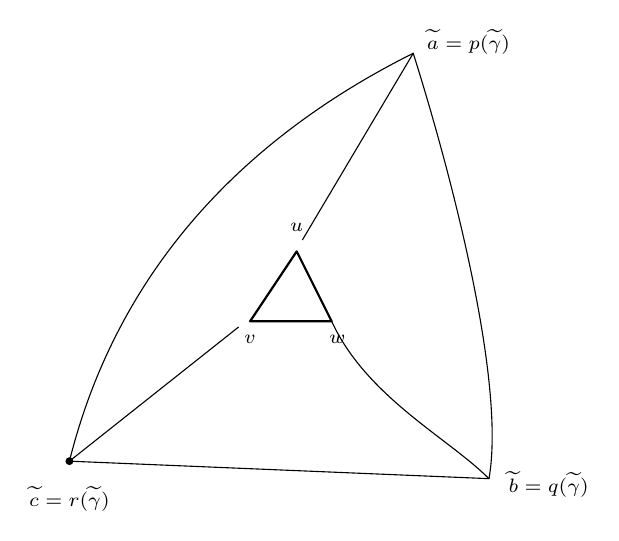
\begin{tikzpicture}[x=0.074cm,y=-0.074cm,line cap=round,line join=round,line width=.4pt]
\draw (59,0) .. controls (29,15) and (8,38) .. (0,70);
\draw (0,70) -- (72,73);
\draw (72,73) .. controls (75,56) and (65,19) .. (59,0);
\draw[thick] (39,34) -- (31,46) -- (45,46) -- cycle;
\draw (59,0) -- (40,32);
\draw (0,70) -- (29,47);
\draw (45,46) .. controls (51,59) and (65,66) .. (72,73);
\fill (0,70) circle[radius=0.05cm];
\node[inner sep=.55pt,anchor=west,font=\scriptsize] at (61,-2) {$\widetilde a=p(\widetilde\gamma)$};
\node[inner sep=.55pt,anchor=west,font=\scriptsize] at (75,74) {$\widetilde b=q(\widetilde\gamma)$};
\node[inner sep=.55pt,anchor=north,font=\scriptsize] at (0,74) {$\widetilde c=r(\widetilde\gamma)$};
\node[inner sep=.55pt,anchor=south,font=\scriptsize] at (39,31) {$u$};
\node[inner sep=.55pt,anchor=north,font=\scriptsize] at (31,48) {$v$};
\node[inner sep=.55pt,anchor=north,font=\scriptsize] at (46,48) {$w$};
\end{tikzpicture}%
}}
\end{tikzcd}%
}

\[\begin{aligned}ayz^{-1}&=1\\x^{-1}bz&=1\\xy^{-1}&\ \unsure{=1}\end{aligned}\]

\[
(a,b,c)\qquad abc=1\quad c=b^{-1}a^{\unsure{-|-1}}
\]
\[
abc=1\qquad
\left.\begin{aligned}ayz&=1\\xbz&=1\end{aligned}\right\}\ \overset{?}{\Downarrow}
\quad xyc=1\qquad\text{i.e.}
\]

\[
\begin{aligned}
ay&=xb\qquad y=a^{-1}xb\\xy&=xa^{-1}xb\\bca&=1\\x^{-1}ayca&=1
\end{aligned}
\]

\[
\begin{aligned}
&\deleted{xyz=}\qquad z=(ay)^{-1}\\
&x=(bz)^{-1}=z^{-1}b^{-1}=ayb^{-1}\deleted{=ayca}\\
&?\Downarrow\quad y=x^{-1}c^{-1}=by^{-1}a^{-1}c^{-1}
=\deleted{\unsure{by^{-1}b|byc^{-1}b}}\ b\deleted{\unsure{(cay)^{-1}}}\\
&\qquad\deleted{\unsure{x=cy(yaby^{-1})}}\\
&\qquad=by^{-1}b^{\unsure{a|1|-1}}=\operatorname{int}(b)y^{-1}
\end{aligned}
\]

\[
\begin{aligned}
&b\,(by^{-1}b^{-1}\qquad\qquad \deleted{c^{-1}y^{-1}}\qquad aby^{-1}=ayb^{-1}\\
&\operatorname{int}(b)\bigl(\operatorname{int}(b)y^{-1}\bigr)^{-1}
\qquad b(by^{-1}b)^{-1}b\\
&\operatorname{int}(b)\,(\operatorname{int}(b)(y))\qquad
b\,b^{-1}yb^{-1}b\qquad by^{-1}=yb^{-1}\qquad (by^{-1})^2=\underline{1}
\end{aligned}
\]

% archive sheet number: 104
